\chapter{Primitive Asimmetriche}
La Crittografia Simmetrica parte dal presupposto che i due interlocutori possiedano una chiave condivisa segreta. Tuttavia, questo non è facilmente realizzabile poiché servirebbe un canale sicuro e, come già ben sappiamo, non esiste. L'idea alla base della crittografia asimmetrica è quella di avere due chiavi una \textbf{pubblica} per cifrare e l'altra \textbf{privata} per decifrare. Una proprietà fondamentale che devono possedere queste due chiavi è che da una non si possa ricavare l'altra in maniera efficiente e viceversa. Dunque, ora più che mai, è importante fare riferimento alla \textbf{teoria della complessità} per renderci conto di quanto l'avversario\footnote{Ricordiamoci che deve sempre essere limitato} possa o meno effettuare l'attacco.
Ci baseremo sull'utilizzare algoritmi che sfruttano operazioni efficienti ma che sia intrattabile effettuare l'operazione inverse.\footnote{In assenza di chiave privata}

Informalmente, si tratta di funzioni facili da calcolare ma difficili da invertire. Per quanto riguarda la facilità di calcolare la funzione, vuol dire che:
\[\exists A : \forall x \in D, A(x,f)=f(x)\]
Mentre, per il fatto che debba essere difficile invertire la funzione, vuol dire che:
\[\nexists A\text{ polinomiale }: A(y,f)=z, f(z)=y\]
Per essere più formali:
\begin{itemize}
    \item Diciamo che $\mu$ è \textbf{trascurabile} se $\forall c \geq 0 \quad \exists k_c : \mu(k) \leq k^{-c}$.
    \item Una funzione $f:\{0,1\}*\xrightarrow{}\{0,1\}*$ è \textbf{unidirezionale} se:
        \begin{enumerate}
            \item Esiste un algoritmo efficiente (PPT) che su input x calcola $f(x)$.
            \item Per ogni algoritmo A, esiste una funzione $\mu_A$ tale che, per k sufficientemente grande:
            \[Pr[f(z)=y : x\in_R\{0,1\}^k;f(x)=y; A(k,y)=z]\leq \mu_A(k)\]
            cioè vuol dire che la probabilità di invertire la funzione è trascurabile.
        \end{enumerate}
\end{itemize}
Per la definizione appena data, A non è ancora capace di invertire la funzione, o meglio, nessuno lo è. Inoltre, non è ancora stato provato che esistano delle funzioni unidirezionali.

Supponiamo adesso di avere una funzione \textbf{unidirezionale trapdoor}, ossia una funzione unidirezionale per cui se posseduta una certa informazione, allora è facile da invertire. Supponendo di prendere delle permutazioni trapdoor, allora sarebbe possibile costruire dei cifrari in modo piuttosto semplice:
\begin{figure}[H]
    \centering
    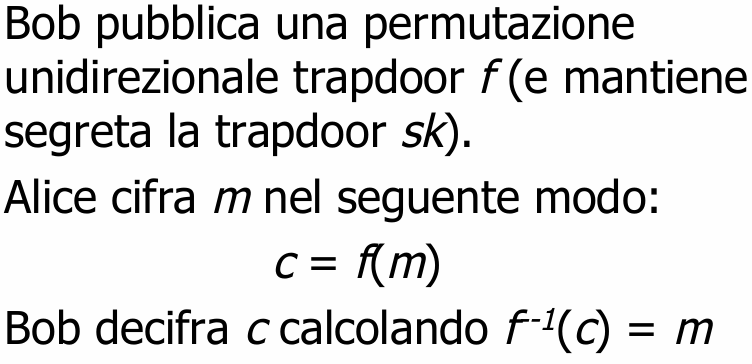
\includegraphics[width=0.5\linewidth]{Images/cifrari_asimmetrici/permutazione_trapdoor.png}
\end{figure}
Attenzione, a questo punto la funzione non è ancora randomizzata, tuttavia a questo ci arriveremo più avanti.

A questo punto ci vengono in aiuto alcuni problemi detti \textbf{NP-completi}, questa particolare categoria di problemi possiede la caratteristica per cui, se la soluzione è data, questa è facilmente intuibile, tuttavia calcolarla de 0 è un problema intrattabile.  
\section{Un po' di Algebra}
Prima di procedere con la spiegazione, è bene fare un po' di ripasso riguardo ad alcuni concetti algebrici che, però, non saranno oggetto d'esame. 
Definiamo $Z_N = \{x:0\leq x < N\}$ e definiamo l'operazione somma come $a,b \in N, a+b \mod N$ che gode di proprietà associativa e presenta l'elemento neutro per cui $a+l=a$ e l'inverso $a+a' = 0 \mod N$. Questo è, quindi, un gruppo additivo.

Ora, dato $Z'_N = \{0 < i < N: gcd(i,N) = 1\}$ dove "gcd" rappresentai l massimo comune divisore, per cui, $Z'_N$ è l'insieme dei numeri coprimi tra i e N. Ad esempio:
\[Z'_{15} = \{1,2,4,7,8,11,13,14\}\]
Possiamo qui definire l'operazione moltiplicazione modulo N come $a,b \in Z'_N, a*b = c \mod N$. Questa operazione si può dimostrare rimanere sempre nello stesso insieme. Diciamo che l'inverso è $a': a *a' = 1 \mod N$. Ad esempio, l'inverso di 1 in $Z_{15}'$ è 1, di 2 è 8 e così via.
Questo è un gruppo moltiplicativo. 

Preso G un gruppo, diremo che $|G| = m$ è l'ordine del gruppo e si può dimostrare che $\forall a \in G, a^m = 1$. Questa notazione varrà per entrambi i gruppi con la differenza che in uno faremo la moltiplicazione per se stesso m volte, nell'altro la somma con se stesso per m volte. Inoltre, se prendiamo S un sottogruppo di G, l'ordine di S divide G, cioè, mantiene le stesse proprietà. 

Per quanto riguarda i costi, normalmente ignoriamo quelli delle operazioni di base, tuttavia, nei sistemi crittografici dove abbiamo numeri con migliaglia di bit, non possiamo farlo. Tra le varie operazioni, abbiamo:
\begin{itemize}
    \item $a \mod N$, costa $O(|a||N|)$.
    \item $a+b$, per due interi a k bit, richiede $O(k)$.
    \item $a*b$, ha costo $O(k^2)$.
    \item $a^m \mod N$ ha costo $O(|m|k^2)$.
\end{itemize}

Per quanto riguarda il trovare il massimo comune divisore, si fa' uso dell'\textbf{algoritmo di Euclide ricorsivo} per cui:
\begin{figure}[H]
    \centering
    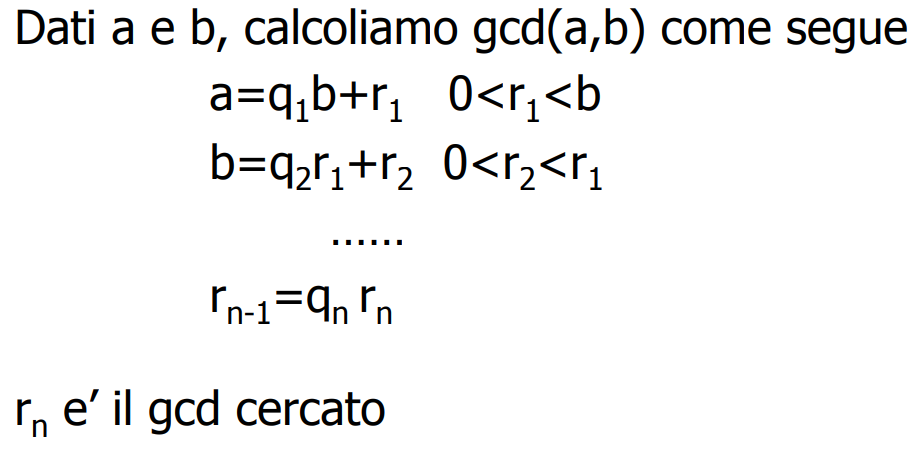
\includegraphics[width=0.6\linewidth]{Images/cifrari_asimmetrici/algoritmo_euclide.png}
\end{figure}

Si può dimostrare che $gcd(a,b)$ è il più piccolo intero positivo nell'insieme $Z_N$, per cui, dato che $gcd(a,b)=1$, essendo a e b \textbf{coprimi} in $Z_N$, possiamo facilmente calcolare l'inverso di a. Per fare ciò, sfruttiamo il fatto che ${\lambda a+ \mu b: \lambda, \mu \in Z}$, da cui:
\begin{align*}
    &\lambda a +\mu N = 1\\
    &\lambda a = 1-\mu N
\end{align*}
Cioè, $\lambda a $ è distante 1 da un multiplo di N e questo vuol dire che $\lambda a \cong 1 \mod N$, ossia $\lambda$ è l'inverso di a. $a \in Z_p*$ è invertibile se $gcd(a,p)=1$, cioè, solo se sono coprimi. 
Dato che vi è questa congruenza, è possibile applicare il \textbf{Teorema Cinese del Resto}:
\begin{figure}[H]
    \centering
    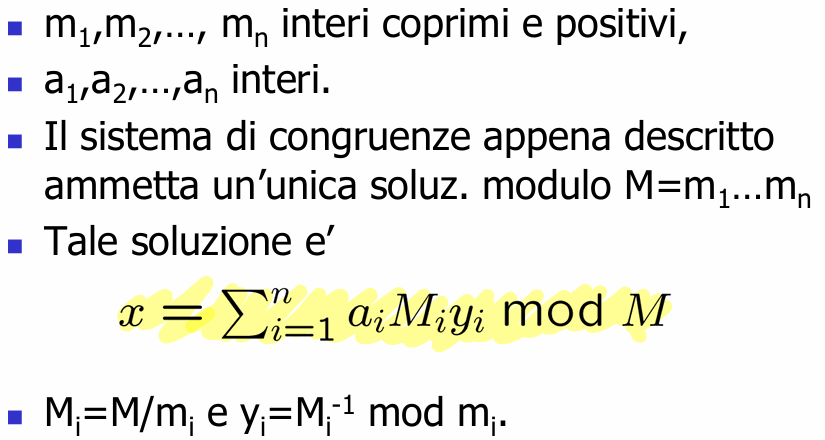
\includegraphics[width=0.6\linewidth]{Images/cifrari_asimmetrici/teorema_cinese_del_resto.png}
\end{figure}
Preso G un \textbf{gruppo}, $m=|G|$ è l'ordine di G. Se $g \in G$, l'ordine di g è il minimo n tale che $g^n=1$ e, se l'ordine di g è proprio m, allora g è detto \textbf{generatore} e, se G ammette un generatore, allora questo è \textbf{ciclico}.

Preso un valore $a \in G$, questo è detto \textbf{quadrato residuo} se esiste $b \in G: b^2 = a$. Detto in parole semplici, di a si può fare la radice quadrata trovando numeri interi. L'insieme dei quadrati residui è un sottogruppo di G. Ci interesseremo particolarmente a guardare $G= Z_p*$ dove p è primo. Definiamo come \textbf{simbolo di Legendre} la funzione tale $J_p : Z \rightarrow \{-1,0,1\}$ nel seguente modo:
\begin{figure}[H]
    \centering
    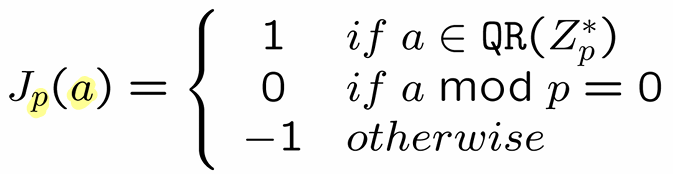
\includegraphics[width=0.4\linewidth]{Images/cifrari_asimmetrici/legendre.png}
\end{figure}
Per i quadrati residui varranno le seguenti cose:
\begin{itemize}
    \item $p>2$ primo, g generatore di $Z_p*$, allora $|QR(Z_p*)| = \frac{p-1}{2}$. Ciò segue dal fatto che $Z_p*$ è composto da $p-1$ elementi poiché:
    \[Z_p* = \{x: 0<x<p \cap gcd(x,p)=1\}=\{0,\dots,p-1\}\]
    Essendo i quadrati tutti della forma $g^{2i} = g^t: t=1,\dots, p-1$, noi di questi dobbiamo considerare solo i pari, per cui avremo $\frac{p-1}{2}$.
    \item $p>2$ primo e $a \in Z_p*$, $J_p(a) = a^{\frac{p-1}{2}\mod p}$. Anche questo si può facilmente dimostrare testando la formula nei vari casi.
    \item $p>2$ primo, segue che per ogni generatore avremo che $g^{\frac{p-1}{2}=-1 \mod p}$.
\end{itemize}
Il problema di $Z_p*$ è che per utilizzarlo abbiamo bisogno di avere a disposizione numeri di moltissimi bit e ciò non è ovviamente conveniente per ciò che abbiamo bisogno di fare. Possiamo, invece, utilizzare le \textbf{curve ellittiche} a patto di utilizzare una matematica estremamente complessa ma ottenendo le proprietà che ci interessano utilizzando molti meno bit.

\section{Primitive Asimmetriche}
Proprio in crittografia simmetrica abbiamo utilizzato i cifrari a blocchi per derivare tutto, dobbiamo procurarci strumenti simili per la crittografia asimmetrica. Per fare ciò, come dicevamo, legheremo le nostre primitive a problemi di natura matematica di cui abbiamo un'operazione facile da calcolare ma di cui è intrattabile riuscire a fare l'inverso.

Primo tra tutti è il \textbf{Logaritmo discreto}. Sia $|G|=m$ un gruppo ciclico e sia $g$ un generatore, il logaritmo discreto $DLog_{G,g}: G \rightarrow Z_m$ è definito come:
\[DLog_{G,g}(a)=x : g^x = a \]
Questa funzione si congettura essere unidirezionale. Il fatto che il problema risulti intrattabile è perché non abbiamo alcun tipo di ordinamento nella sequenza di risultati di a. Possiamo definire il problema del logaritmo discreto come:
\begin{figure}[H]
    \centering
    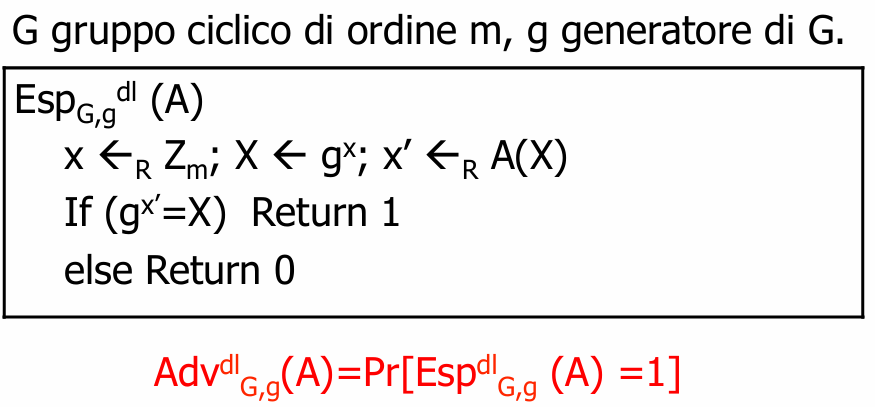
\includegraphics[width=0.5\linewidth]{Images/cifrari_asimmetrici/problema_dl.png}
\end{figure} 
Dove G,g sono noti all'avversario e questo ha come obiettivo quello di indovinare, a partire da $X$ il valore $x: g^x = X$. Diciamo che è un problema DL intrattabile se il vantaggio dell'attaccante è prossimo a 0 per ogni avversario computazionalmente limitato.
Ipotizziamo che per alcuni specifici gruppi il logaritmo discreto sia intrattabile, vediamo il \textbf{problema Diffie-Hellman computazionale}. Questo problema deriva dalla procedura di scambio delle chiavi definita da Diffie-Hellman che è la seguente:
\begin{figure}[H]
    \centering
    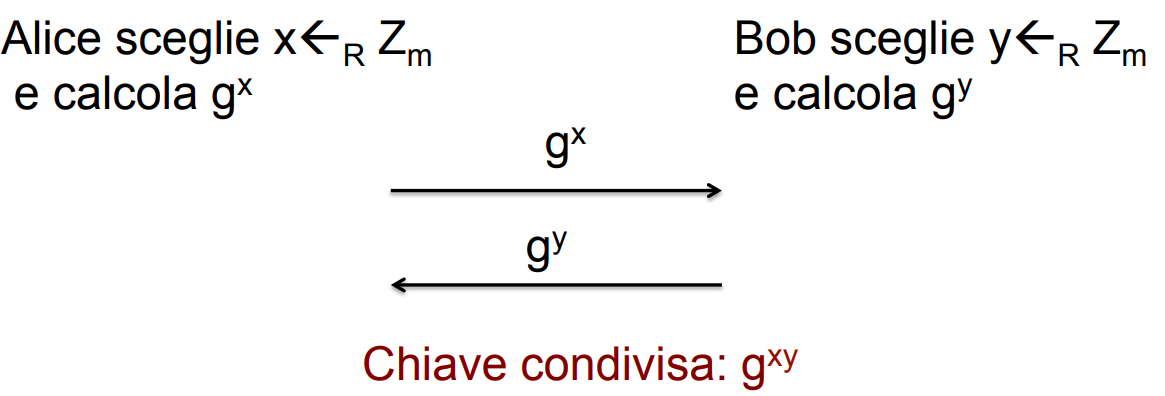
\includegraphics[width=0.5\linewidth]{Images/cifrari_asimmetrici/diffie_hellman.png}
\end{figure} 
Da qui possiamo definire il seguente esperimento:
\begin{figure}[H]
    \centering
    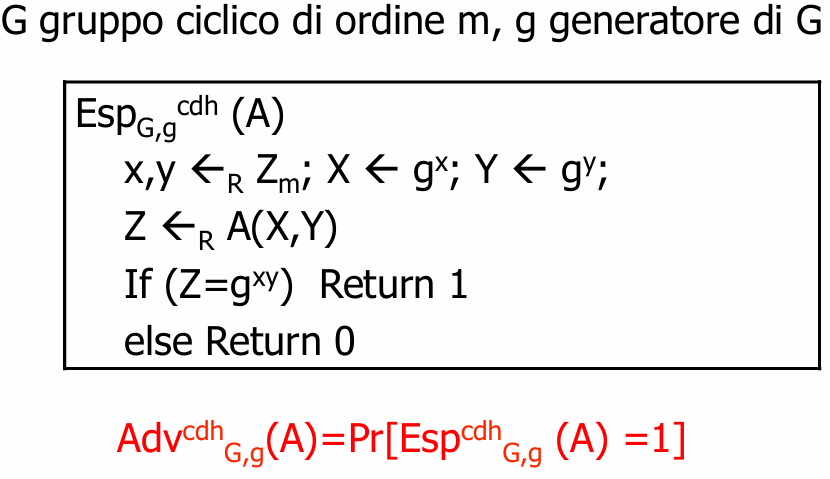
\includegraphics[width=0.5\linewidth]{Images/cifrari_asimmetrici/esperimento_cdh.png}
\end{figure} 
Per cui, il problema è intrattabile se il vantaggio dell'avversario è prossimo a zero per ogni avversario computazionalmente limitato. È chiaro che:
\[Adv^{dl}_{G,g}(A)\leq Adv^{cdh}_{G,g}(A)\]
E, dunque, il solo modo che abbiamo per risolvere il problema CDH è proprio quello di risolvere il problema DL.
Tuttavia, per garantire che la scelta della chiave condivisa sia davvero random, possiamo definire il seguente esperimento:
\begin{figure}[H]
    \centering
    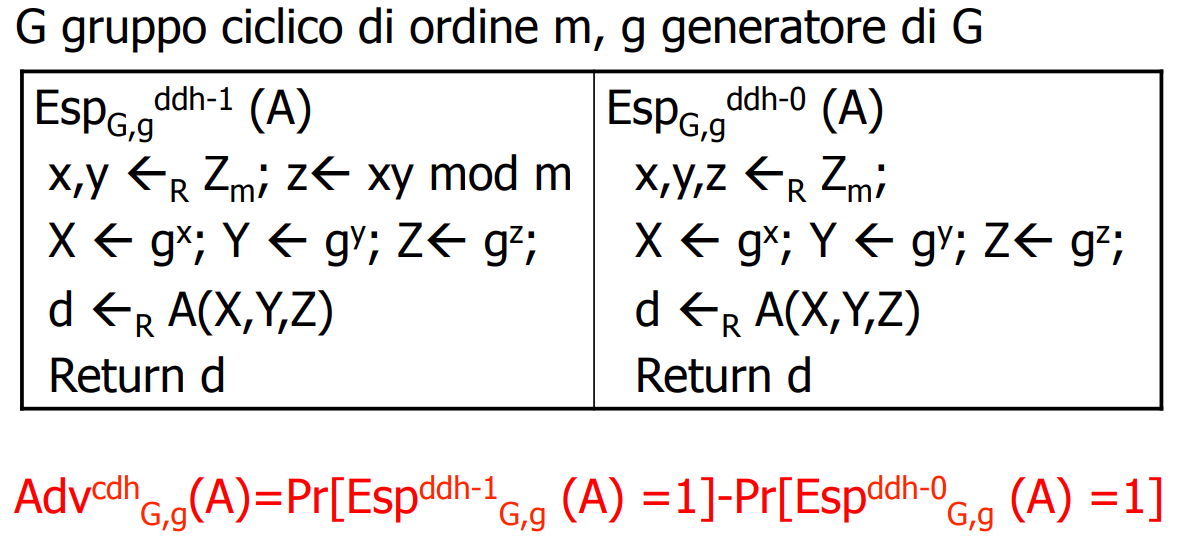
\includegraphics[width=0.5\linewidth]{Images/cifrari_asimmetrici/decisional_diffie_hellman.png}
\end{figure} 
Che è detto \textbf{problema decisionale Diffie-Hellman}. La chiave viene scelta random se il vantaggio dell'avversario è prossimo a zero per ogni avversario computazionalmente limitato. Possiamo dimostrare che:
\[Adv^{cdh}_{G,g}(A)\leq Adv^{ddh}_{G,g}(A) + \frac{1}{|G|}\]
Cioè che il problema DDH non può essere più difficile di CDH:
\begin{figure}[H]
    \centering
    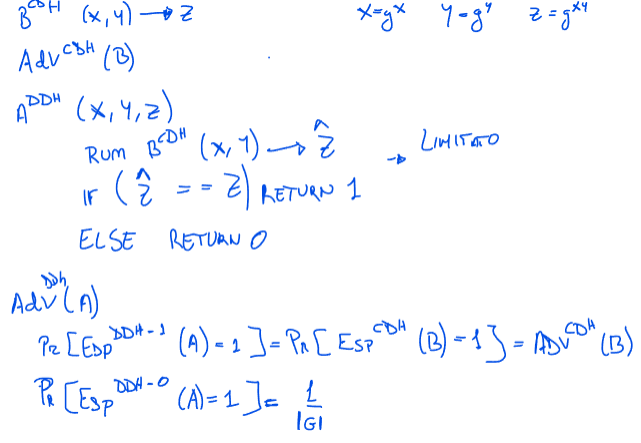
\includegraphics[width=0.5\linewidth]{Images/cifrari_asimmetrici/cdh_minore_ddh.png}
\end{figure} 
Nonostante ciò, abbiamo che, in realtà, il problema decisionale Diffie-Hellman non è intrattabile in $Z_p*$ questo perché, come vedremo tra poco, esiste un attacco basato sul \textbf{simbolo di Legendre}. Questo si basa sul fatto che, in $Z_p*$, alcune proprietà relative a questo numero, rimangono anche dopo la moltiplicazione. Per cui:
\begin{figure}[H]
    \centering
    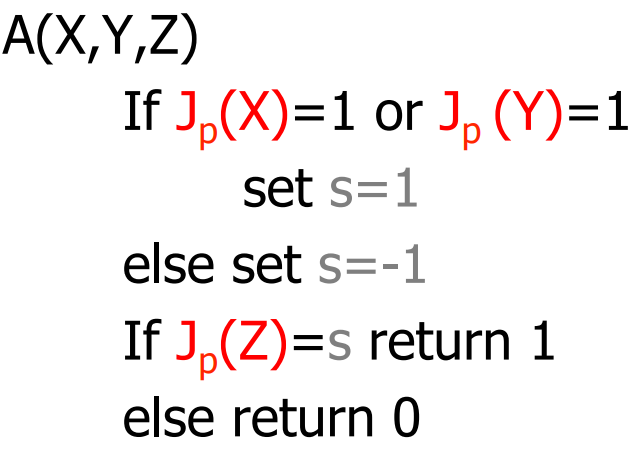
\includegraphics[width=0.4\linewidth]{Images/cifrari_asimmetrici/attacco_legendre.png}
\end{figure} 
E ciò si può dimostrare nel seguente modo:
Se $Z = g^{xy} = g^{x^y}$, ma se per $g^x,g^y$ vale che $J_a(X) = 1, \quad J_a(Y)$, allora la moltiplicazione sarà una cosa del tipo $g^{2x'^{y}}$ che è un quadrato residuo, cioè $J_a(Z) = 1$, altrimenti, se nessuno dei due lo è, allora $J_a(Z) = -1$. Calcoliamo il vantaggio di questo attaccante:
\[Avd(A)^{ddh} = Pr[Esp^{ddh-1}(A)=1]-Pr[Esp^{ddh-0}(A)=1]=1-1/2 = 1/2\]
La probabilità che nell'esperimento $ddh-0$ A dica 1 è uguale alla probabilità che fissato 1 (che può essere o 1 o -1), a caso becchiamo un numero che rende l'if binario vero.

Una cosa parecchio importante che vedremo, è che a noi servono specifici numeri primi per cui i fattori della sua fattorizzazione sono grandi abbastanza per cui non possiamo risolverli in maniera efficiente tramite il teorema cinese del resto. Vengono considerati dei buoni numeri primi quelli della forma $p = 2q +1 $ dove $q$ è un numero primo molto grande e che, quindi, non può essere attaccato mediante l'algoritmo Pohlig-Hellman.

\section{Calcolare Logaritmi Discreti}
I migliori modi per calcolare i logaritmi discreti, sono principalmente di 2 tipi:
\begin{enumerate}
    \item \textbf{Index Calculus}: sono metodi piuttosto efficienti che però richiedono la presenza di specifiche proprietà aritmetiche per funzionare.
    \item \textbf{Collision Search}: metodi generici che hanno, però, complessità esponenziale.
\end{enumerate}
Di questi vedremo l'algoritmo \textbf{Pohlig-Hellman} che è del primo tipo e l'algoritmo \textbf{Baby-step Giant-Step (Shanks)} che è del secondo tipo.
\subsection{Baby-Step Giant-Step}
Questo algoritmo prende in input $g$ un generatore di $G$ e $X$ un elemento in $G$, e dà in output $x: g^x = X$. Supponiamo che $|G| = m, n = \lceil \sqrt{m} \rceil$. Allora, possiamo porre $x = nx_1 + x_0$ con $ 0 \leq x_1,x_0 \leq n$, così facendo, noi cerchiamo due numeri anziché uno solo, il ché è molto più facile per trovare $X=g^{nx_1+x_0} \rightarrow Xg^{-x_0} = (g^n)^{x_1}$

Per fare ciò l'algoritmo agisce in questo modo:
\begin{figure}[H]
    \centering
    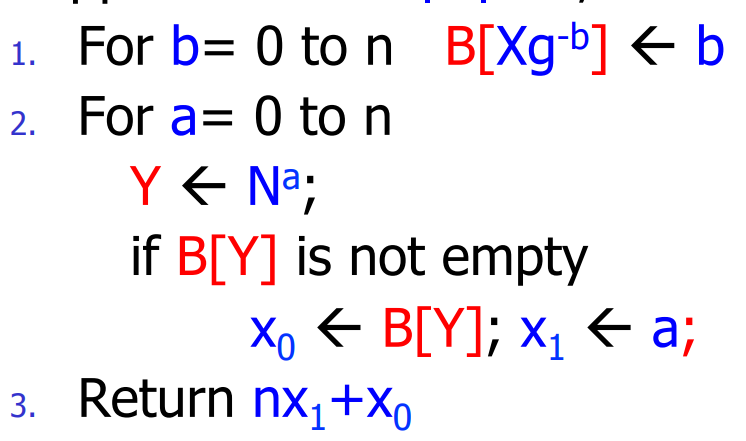
\includegraphics[width=0.4\linewidth]{Images/cifrari_asimmetrici/baby_step_giant_step.png}
\end{figure} 
Il primo ciclo for rappresenta i \textbf{baby-step} in cui l'algoritmo calcola prima tutti i lati a sinistra dell'equazione sopra e farà $\sqrt{m}$ passi e, dopodiché farà i \textbf{giant step}\footnote{È considerato giant perché qui abbiamo salti più lunghi nell'array.} in cui calcolerà tutti i lati a destra dell'equazione e, se trova la posizione occupata, allora abbiamo trovato la collisione e siamo riusciti a rompere il logaritmo discreto. 
La complessità di questo algoritmo è, quindi $\sqrt{m}$, tuttavia abbiamo la necessità di avere array molto grandi anche se ciò, in realtà, non è un grosso problema dato che lo spazio è riutilizzabile.

\subsection{Pohlig-Hellman}
Questo algoritmo funziona solo nel caso in cui la fattorizzazione di $p-1$ è nota. Questo algoritmo, prende in input $X$, $g$ il generatore in $G$ e la fattorizzazione di $p-1$ Infatti, si possono calcolare $DL$ in tempo:
\[\sum_{i=1}^{n} a_i (\sqrt{p_i}+|p_i|)\]
Per fare ciò, seguiamo questo ragionamento:
\begin{figure}[H]
    \centering
    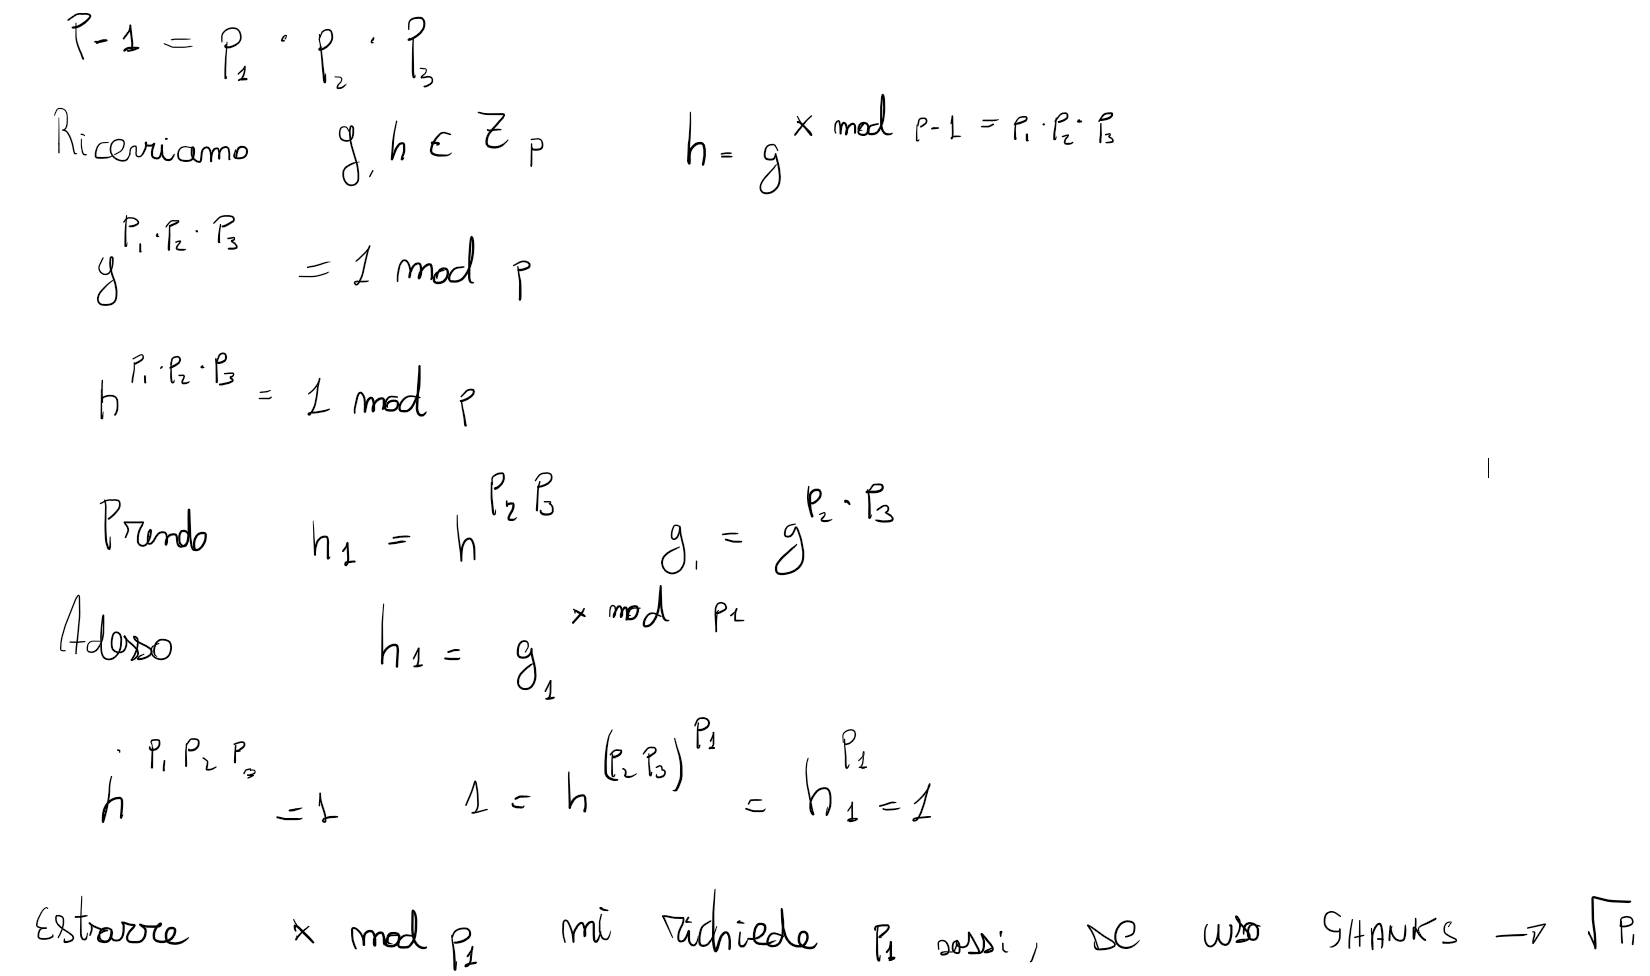
\includegraphics[width=0.85\linewidth]{Images/cifrari_asimmetrici/pohlig_hellman/1.png}
\end{figure} 
\begin{figure}[H]
    \centering
    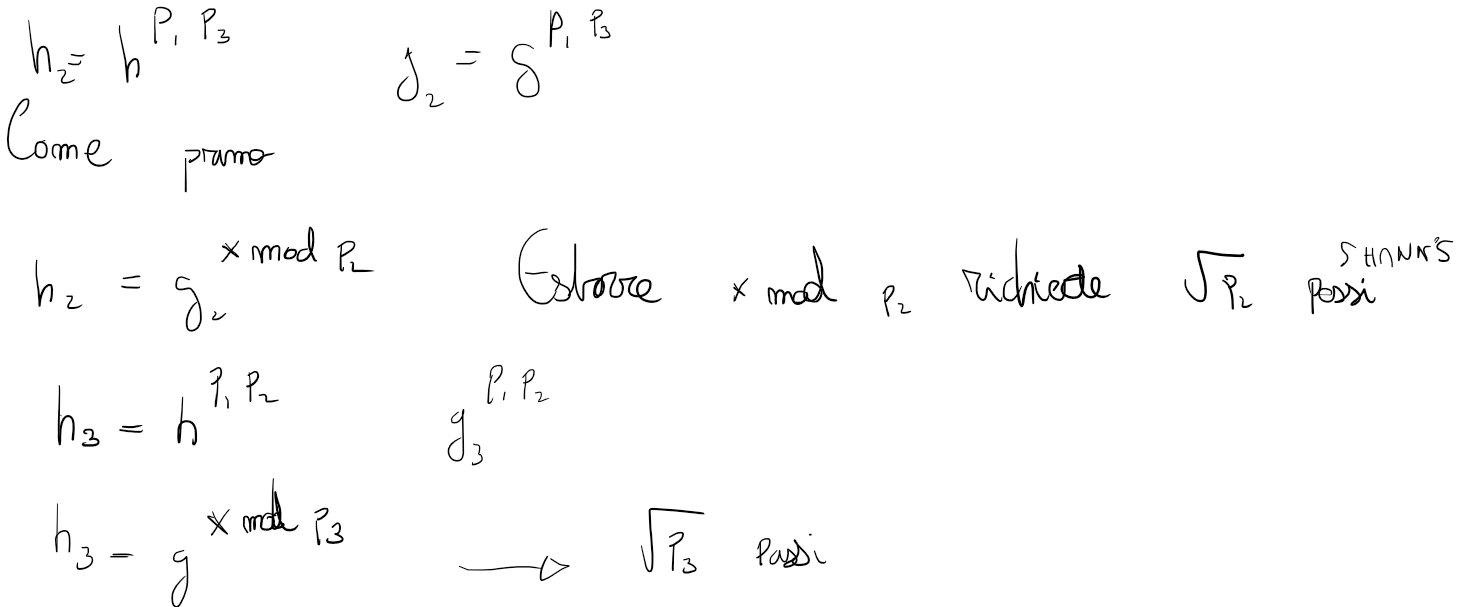
\includegraphics[width=0.85\linewidth]{Images/cifrari_asimmetrici/pohlig_hellman/2.png}
\end{figure} 
A questo punto, siamo riusciti a calcolare in tempo $\sqrt{p_1} + \sqrt{p_2}+\sqrt{p_3}$, dunque, abbiamo calcolato $a_i = x \mod p_i$ con $p$ che sono tutti coprimi tra loro. Dunque, possiamo utilizzare il teorema del resto cinese per calcolare $x \mod p_1 p_2 p_3$. Da qui, segue quanto detto prima: Se $p_1, p_2, p_3$ sono piccoli (es. 10 cifre), i calcoli sono immediati. Se invece $p-1 = 2q$ con $q$ enorme, questo trucco non serve a nulla perché fare brute forcing su $\sqrt{q}$ resta impossibile da calcolare.

\section{Problema della Fattorizzazione}
Sia $P^k$ insieme dei primi di taglia $k$.
\[f:P^k \times P^k \rightarrow N, f(p,q)=pq\]
Cioè, p e q rappresentano la fattorizzazione di N. L'algoritmo più rapido conosciuto per fare ciò è \textbf{Number Field Sieve} che ha complessità superpolinomiale. Oggi, fattorizzare numeri di 2048 bit è considerato intrattabile.
\subsection{RSA}
Sia N il prodotto di due primi $p,q$ e $e$ un esponente pubblico. La funzione RSA è definita come:
\[RSA[N, e](x) = x^e \mod N\]
Questa è la prima \textbf{funzione trapdoor} per cui, dati $e,N$ e $y =x^e \mod N$, è possibile ritrovare x solo se si ha la conoscenza di $p,q$.
Sia $N=pq$, consideriamo il gruppo $Z_N*$ tale che: 
\[Z_N* = \{x: x<N \cap gcd(x,N)=1\}=\{0,\dots,N-1\}\]
Il gruppo ha ordine $\varphi(N)= (p-1)(q-1)$, dunque per il Teorema di Eulero $x^{\varphi(N)} \equiv 1 \pmod N$.\footnote{$\varphi$ indica la funzione totiente di Eulero, legata alla fattorizzazione di N.}

Applicando l'algoritmo di Euclide esteso a $(e, \varphi(N))$, sappiamo che esistono interi $\lambda,\mu$ tali che $\lambda e + \mu \varphi(N)=1$. Per coerenza con la letteratura RSA, poniamo $\lambda = d$.

Questo ci permette di calcolare l'inverso modulare $d$ tale che:
\[ ed \equiv 1 \pmod{\varphi(N)} \]

Possiamo ora dimostrare la correttezza dell'algoritmo.
Dato il messaggio cifrato $y = x^e \mod N$, per recuperare $x$ calcoliamo:

\begin{align*}
    y^d &\equiv (x^e)^d \pmod N \\
    &\equiv x^{ed} \pmod N \\
    &\equiv x^{1+k\varphi(N)} \pmod N && \text{\small(poiché $ed - 1$ è multiplo di $\varphi(N)$)}\\
    &\equiv x \cdot (x^{\varphi(N)})^k \pmod N \\
    &\equiv x \cdot (1)^k \pmod N && \text{\small(sostituendo $x^{\varphi(N)} \equiv 1$)}\\
    &\equiv x \pmod N
\end{align*}
Dunque, se conosco $N=pq$, posso:
\begin{enumerate}
    \item Calcolare $\Phi(N) = (p-1)(q-1)$
    \item Usare l'algoritmo esteso di Euclide su $(e, \Phi(N))$ per trovare d. 
    \item Utilizzare d per invertire $y$.
\end{enumerate}

La domanda che ci poniamo adesso è, se io riesco a risolvere il problema RSA, posso risolvere anche il problema della fattorizzazione? Ci sono vari casi da tenere in considerazione:
\begin{enumerate}
    \item Supponiamo di avere un algoritmo $E_1$ che dato N calcola $\Phi(N)$, cioè $E_1(N) \rightarrow \varphi(N)$,allora ho risolto il problema della fattorizzazione.
    \item Supponiamo di avere un algoritmo $E_2(N, e)\rightarrow d$, allora da questo algoritmo posso ricavare $ed = 1+\varphi(N)$ e, quindi, $ed -1 = t\varphi(N)$, e, quindi, calcolare la chiave dato che sappiamo che $ed-1$ è di sicuro un multiplo di $\varphi(N)$.
    \item Se abbiamo, invece, $E_3(N,e,y)\rightarrow x$ abbiamo effettivamente risolto RSA, tuttavia non possiamo concludere nulla riguardo alla fattorizzazione di N. Dunque, i due problemi non sono equivalenti.
\end{enumerate}
A questo punto abbiamo alcuni problemi di natura matematica che dobbiamo tenere in considerazione:
\begin{enumerate}
    \item Abbiamo abbastanza numeri primi?
    \item Supponendo che ve ne siano abbastanza, come faccio a dire che per ogni "dimensione" ci sono abbastanza numeri primi da non permetterci di scegliere contemporaneamente lo stesso?
\end{enumerate}
La risposta alla prima domanda è sì e deriva da una dimostrazione per assurdo effettuata dal matematico Euclide.
Alla seconda domanda, invece, risponde il \textbf{Prime Number Theorem}:
\begin{figure}[H]
    \centering
    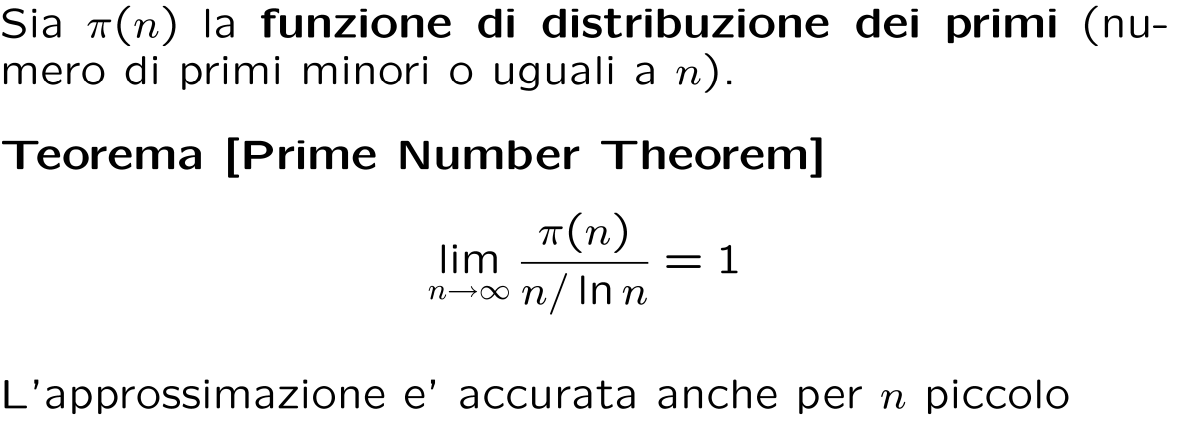
\includegraphics[width=0.5\linewidth]{Images/cifrari_asimmetrici/teorema_numeri_primi.png}
\end{figure} 
Ciò vuol dire che se io prendo un intero a caso tra 1 ed n, allora questo sarà primo con probabilità $1/ln(n)$.
Questo ci rassicura molto, tuttavia, non ci dice nulla sul come capire se un numero è primo o no. Un metodo piuttosto conosciuto è quello basato sul \textbf{crivello di Eratostane} che, tuttavia, non è per nulla efficiente. Utilizziamo, invece, l'algoritmo \textbf{Miller-Rabin}. 
\subsection{Algoritmo Miller-Rabin}
L'idea alla base di questo algoritmo è quella di cercare una prova che il numero in input sia composito. Se il test restituisce \textbf{Composito}, allora la risposta è corretta con probabilità 1, se restituisce \textbf{Primo}, la risposta è sbagliata co probabilità $2^{-2s}$. Per come è costruito l'algoritmo, il testa ha complessità $O(s|a|^3)$, vediamo l'algoritmo:
\begin{figure}[H]
    \centering
    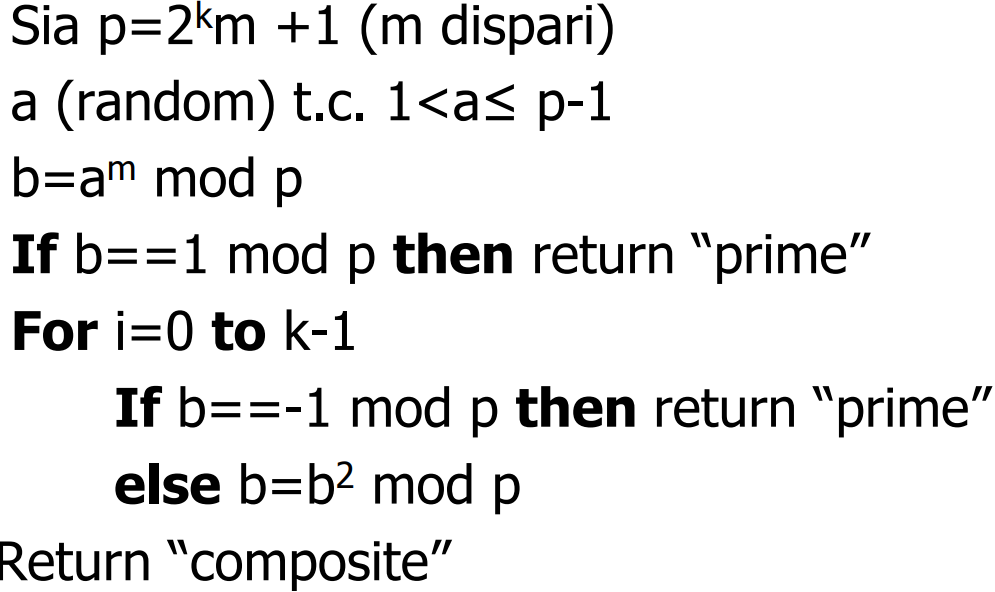
\includegraphics[width=0.5\linewidth]{Images/cifrari_asimmetrici/miller-rabin.png}
\end{figure} 
Dimostriamo che l'algoritmo funziona nel caso in cui p sia primo. Allora, in questo caso, dato che $p-1 = 2^{k}m$, avremo che $a^{2^{k}m} = 1 \mod p$, per cui facciamo di volta in volta la radice quadrata modulo p che potrebbe ritornare due valori che sono o -1 o 1\footnote{Stiamo cercando un numero $x$ tale che $x^2 \equiv 1 \pmod p$ e questo può valere solo per 1 o p-1 nel caso dei numeri primi. Nel caso in cui il numero sia composto, potrebbe valere questa condizione solo per un a particolare, motivo per cui l'algoritmo può sbagliare.}, nel caso in cui dica -1, allora è un numero primo, altrimenti si reitera il processo effettuando nuovamente la radice quadrata fino ad arrivare a $a^{2m} = 1$ e, infine, a $a^m$ che risponderà primo a prescindere dal fatto che il modulo sia 1 o -1.
\begin{figure}[H]
    \centering
    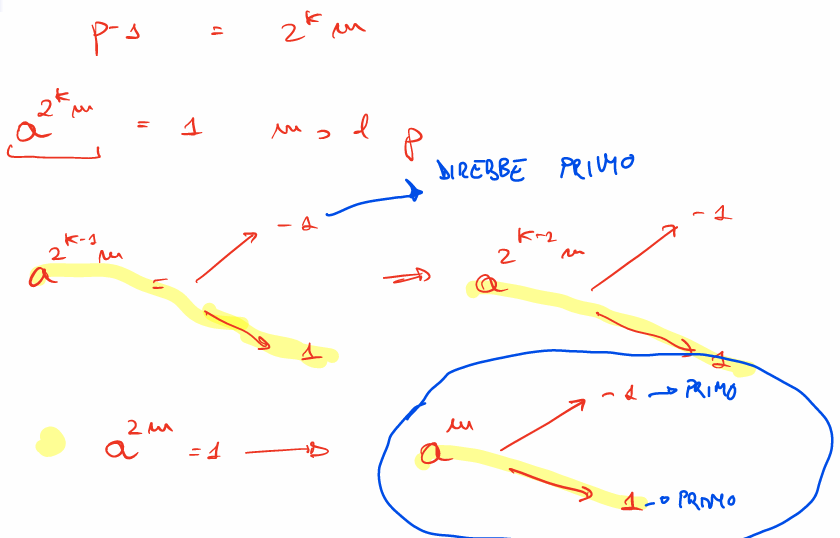
\includegraphics[width=0.5\linewidth]{Images/cifrari_asimmetrici/miller-rabin_2.png}
\end{figure} 

A questo punto la domanda che ci rimane è, come generiamo dei primi del tipo $p=2q+1$, l'unica cosa che possiamo fare è generare dei numeri primi $q$, effettuare $2q+1$ e verificare che $p$ sia primo a sua volta. Per ottimizzare questo processo, genererò solo $q$ dispari ed effettuerò il test di primalità Miller Rabin su $p=2q+1$ solo su candidati che hanno già passato alcuni test per verificare che non siano multipli di 3,5,7 ecc. 

A questo punto ci chiediamo come effettuare l'elevamento a potenza di RSA. Banalmente si potrebbe pensare di agire in maniera ricorsiva mediante il classico algoritmo:
\begin{figure}[H]
    \centering
    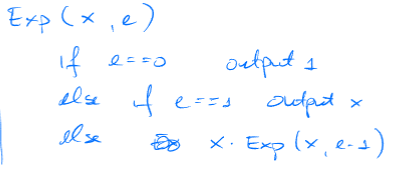
\includegraphics[width=0.5\linewidth]{Images/cifrari_asimmetrici/pow_1.png}
\end{figure} 
Tuttavia, una ottimizzazione che possiamo fare è la seguente:
\begin{figure}[H]
    \centering
    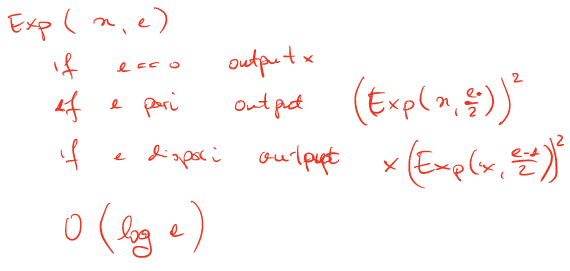
\includegraphics[width=0.5\linewidth]{Images/cifrari_asimmetrici/pow_2.png}
\end{figure} 
Che, come possiamo vedere, ci permette di passare da una complessità $O(e)$ a una $O(log (e))$.
Se volessimo, invece, utilizzare una versione iterativa al posto di quella ricorsiva, esiste il metodo \textbf{Square and Multiply} che parte dall'idea di calcolare $x^e \mod N$ sfruttando la rappresentazione binaria di e. 
\begin{figure}[H]
    \centering
    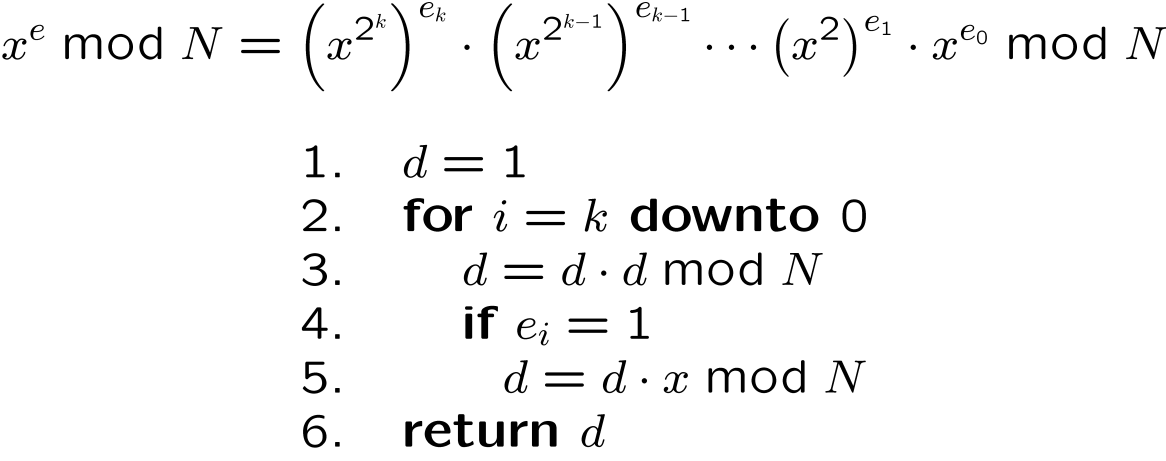
\includegraphics[width=0.5\linewidth]{Images/cifrari_asimmetrici/pow_3.png}
\end{figure} 

\chapter{Cifrari Asimmetrici}
Passiamo adesso finalmente ai cifrari asimmetrici. Sostanzialmente, tutti questi cifrari si basano su Diffie-Hellman e RSA. Come sempre, avremo un algoritmo randomizzato di \textbf{generazione della coppia di chiavi $(sk,pk)$}, un algoritmo randomizzato di Encryption che prende in input una chiave $pk$ e un messaggio $m$ e lo cifra in $C$ e, infine, l'algoritmo di Decryption che da $(sk,C)$ produce $m$.

Una cosa da attenzionare è che messaggi e crittotesti sono elementi di gruppi specifici, per cui, il messaggio iniziale sarà trasformato secondo alcune regole al fine di renderlo parte del gruppo a cui l'algoritmo di cifratura fa' riferimento.

Andiamo a dare la solita nozione di sicurezza che sarà in parte simile a quella già vista ma con alcune piccole differenze. Ad esempio, l'avversario non avrà più bisogno di un oracolo per cifrare i suoi messaggi poiché la chiave sarà pubblica e, quindi, l'avversario potrà farlo da solo. Supporremo che, quindi, l'attaccante farà un solo accesso all'oracolo di cifratura che sarà la domanda della sfida. Definiamo, quindi, l'esperimento \textbf{ind-cpa}, definito nel seguente modo: 
\begin{figure}[H]
    \centering
    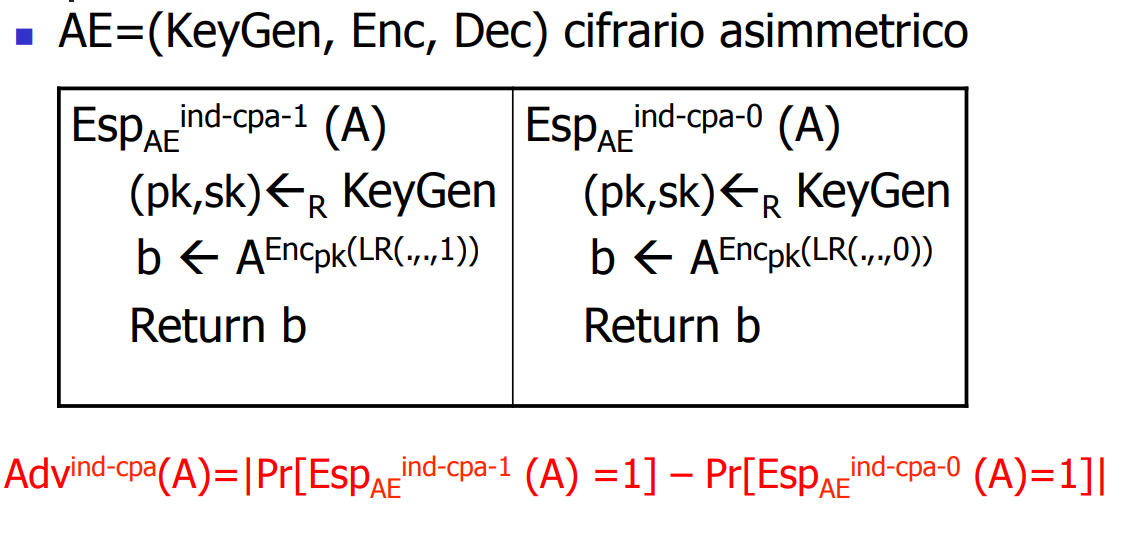
\includegraphics[width=0.5\linewidth]{Images/cifrari_asimmetrici/ind_cpa_asimmetrico.png}
\end{figure}
Anche in questo caso, il cifrario sarà indistinguibile da attacchi cpa se il vantaggio dell'attaccante è prossimo a zero per ogni avversario computazionalmente limitato. A differenza della sua controparte simmetrica, l'esperimento non impone che i due messaggi abbiano la stessa lunghezza poiché le trasformazioni che questi subiscono per entrare nel gruppo, li renderanno comunque con la stessa lunghezza.

Una nozione ancora più forte sarà quella data dall'esperimento \textbf{ind-cca}, cioè, di indistinguibilità da attacchi a crittotesto scelto, ossia, l'attaccante ha a disposizione anche un oracolo di decifratura. Questo esperimento è definito a questo modo:
\begin{figure}[H]
    \centering
    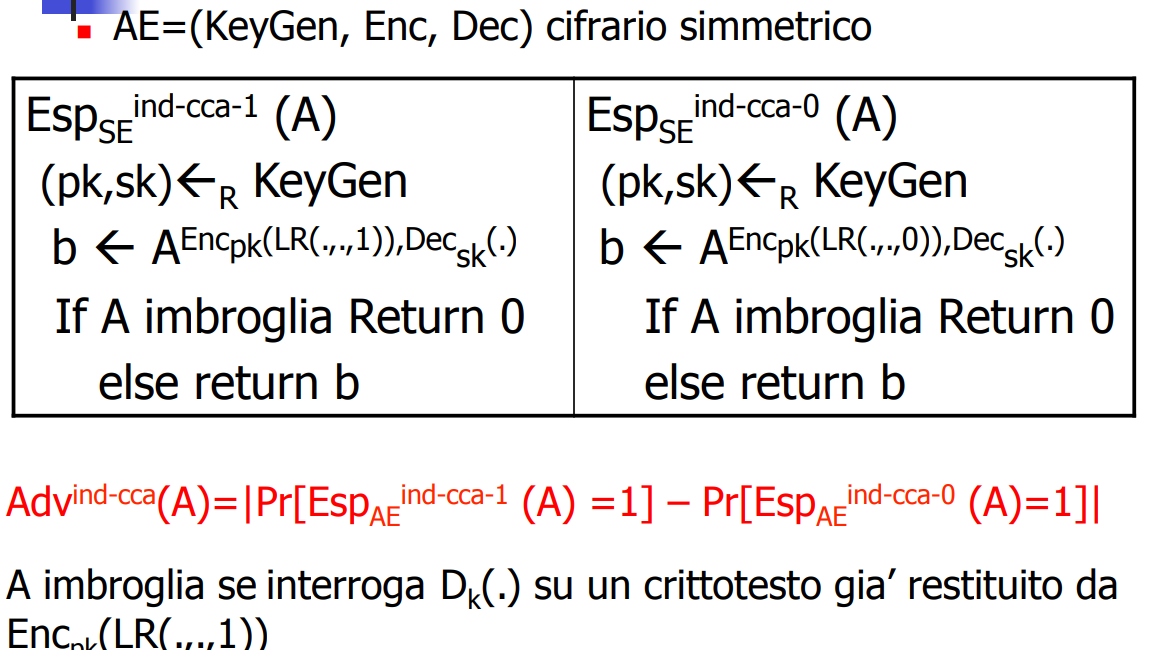
\includegraphics[width=0.5\linewidth]{Images/cifrari_asimmetrici/ind_cca_asimmetrico.png}
\end{figure}

Questo modello è molto più rilevante che nel caso simmetrico e questo è dovuto ad alcune tipologie di attacchi che potremmo adottare:
\begin{itemize}
    \item \textbf{Challenge-Response}: Supponiamo un attaccante chieda in qualche modo alla vittima di dare prova di essere lui. La vittima per fare ciò ha la necessità di tradurre qualcosa con la sua chiave privata. Da qui, segue l'importanza del modello cca poiché spesso si hanno situazioni dove un attaccante può, in un qualche modo, ingannare un server o la stessa vittima per far sì che questo traduca i suoi messaggi.
    \item \textbf{Asta}: Immaginiamo di avere due computer che partecipano a un'asta gestita da un server. Per potervi partecipare, questi dovranno inviare la loro proposta al server in maniera tale che questa sia cifrata con la sua chiave pubblica. Una volta che il server riceve le puntate, questo le decifra e vince la puntata maggiore. Per far sì di avere la vittoria assicurata, un computer potrebbe barare prendendo il messaggio dell'avversario e aggiungendogli tramite alcune trasformate, 1. Così facendo non solo vincerebbe sicuramente l'asta ma riuscirebbe a farlo con il minor dispendio possibile. Questa cosa non è fattibile nel caso in cui un modello sia ind-cca, poiché non si avrebbe modo di conoscere l'effetto delle trasformazioni che effettuiamo. 
\end{itemize}

Il concetto descritto nel caso dell'asta è di particolare interesse ed è una proprietà nota come \textbf{non malleabilità}. Diremo che un cifrario sicuro in senso ind-cca garantisce non malleabilità. Sia $AE = (KeyGen, Enc, Dec)$ un cifrario asimmetrico sicuro in senso ind-cpa. Sia $F: M \rightarrow M$ una funzione efficacemente computabile. Sia AE malleabile relativamente ad F, allora esiste una procedura $MAUL: MAUL(Enc(m),F) \rightarrow Enc(F(M))$. Se un cifrario permette ciò, allora non può essere sicuro in senso ind-cca. Possiamo verificare questa cosa generando il seguente attaccante:
\begin{figure}[H]
    \centering
    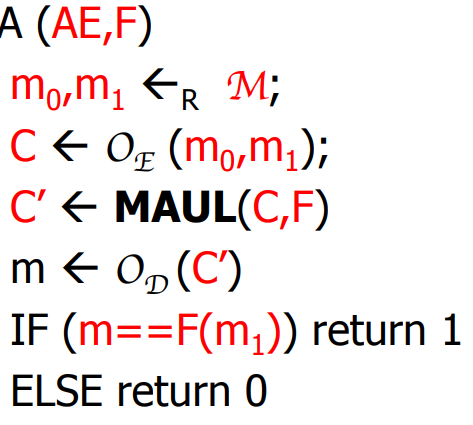
\includegraphics[width=0.3\linewidth]{Images/cifrari_asimmetrici/malleabilita_attaccante.png}
\end{figure}

Andiamo ad analizzare il vantaggio dell'attaccante:
\begin{align*}
    &Pr[Esp^{ind-cca-1}(A)=1]=1 & \text{L'attaccante non può mai sbagliare}\\
    &Pr[Esp^{ind-cca-0}(A)=1]=0
    &\text{Dunque il vantaggio di A sarà}:\\
    &Adv(A)=1
\end{align*}

Nonostante la malleabilità sia un qualcosa che può spaventarci, questa può essere utile in specifici contesti. Un esempio è quello per cui vogliamo effettuare statistica su dati cifrati senza però decifrarli. Contesti del genere possono accadere spesso quando si trattano dati sanitari o magari bancari dove si vogliono rendere anonimi alcuni dati ma si vuole comunque poter effettuare operazioni su di essi. Questa tipologia di cifratura è conosciuta come \textbf{Omomorfica} che è un tipo di crittografia che permette di eseguire calcoli su dati cifrati, ottenendo un risultato cifrato che corrisponde a quello che si otterrebbe se i dati fossero in chiaro.
\section{Hybrid Encryption}
Per quanto possiamo impegnarci a creare cifrature asimmetriche sicure, a causa puramente di aspetti che non possiamo modificare, questa sarà sempre più lenta della cifratura simmetrica. Ragion per cui nascono i \textbf{cifrari ibridi}. Questi sfruttano cifratura simmetrica per la cifratura dei messaggi e cifratura asimmetrica per lo scambio della chiave, di fatto, ottenendo una maggiore velocità e non avendo alcun tipo di problema con la codifica.

Siano $AE=(KeyGen^a, Enc^a, Dec^a), SE=(KeyGen^s, Enc^s, Dec^s)$ rispettivamente un cifrario asimmetrico e uno simmetrico. 

Il cifrario $HE=(KeyGen^H, Enc^H, Dec^H)$ è definito dai seguenti algoritmi:
\begin{itemize}
    \item \textbf{KeyGen$^H$}: Banalmente la generazione della chiave sarà effettuata seguendo l'algoritmo $KeyGen^a$.
    \item \textbf{Enc$^H$}: Qui arriviamo ad alcuni dettagli più interessanti. Questo algoritmo prenderà come input la chiave privata $pk$ e il messaggio $m$ da inviare. Dopodiché verrà generata una chiave simmetrica $k$ con cui verrà cifrato il messaggio e, infine, verrà cifrata la chiave simmetrica mediante cifratura asimmetrica con la chiave privata del destinatario. Così facendo verrà inviato $C^s||C^a$ dove $C^s$ contiene la il messaggio e $C^a$ contiene la chiave simmetrica con cui è stato cifrato il messaggio.
    \begin{figure}[H]
        \centering
        
\includegraphics[width=0.3\linewidth]{Images/cifrari_asimmetrici/hybrid_enc/encrypt.png}
    \end{figure}
    \item \textbf{Dec$^H$}: Quando effettueremo la decifratura del messaggio, avremo a nostra disposizione $sk$ la chiave segreta del destinatario e $C^s,C^a$. Quello che faremo sarà, dunque decifrare $C^a$ per ottenere la chiave simmetrica con cui è stato cifrato il messaggio e, infine, decifrare il messaggio appena ottenuto.
    \begin{figure}[H]
        \centering
        
\includegraphics[width=0.3\linewidth]{Images/cifrari_asimmetrici/hybrid_enc/decrypt.png}
    \end{figure}
\end{itemize}
La chiave simmetrica scambiata tra i due, sarà definita \textbf{chiave di sessione} e questa cambierà, per l'appunto, a ogni nuova sessione. Così facendo, perdendo una chiave di questo tipo, non mettiamo a rischio future sessioni.
\section{Cifrario El-Gamal}
Il cifrario El-Gamal fu uno dei primi cifrari asimmetrici, questo è definito su un gruppo $G$ di ordine $q$ e sia $g$ un generatore di questo gruppo. Possiamo definire El-Gamal in questo modo:
\begin{itemize}
    \item \textbf{KeyGen}: L'algoritmo di generazione della chiave sceglie un x random tra 1 e q e si prende $h = g^x$. La chiave pubblica $pk = (g, h, q)$ mentre la chiave privata è $sk = (x)$.
    \item \textbf{Enc(PK,M)}: L'algoritmo di Encryption genera una randomness $r$ tra 0 e q. Dopodiché pone $C_1 = g^r$ e $C_2 = h^rM$. In questo caso, come possiamo notare non abbiamo alcun tipo di trasformazione del messaggio poiché lo spazio dei messaggi corrisponde proprio al gruppo.
    \item \textbf{Dec(SK,$C_1,C_2$)}: Questo algoritmo prende $A = C_1^x$ e da questo avremo che $M = \frac{C_2}{A}$. Per capire questa cosa, vediamo cosa accade. 
    \begin{figure}[H]
        \centering
        
\includegraphics[width=0.4\linewidth]{Images/cifrari_asimmetrici/El_gamal/correttezza.png}
    \end{figure}
\end{itemize}
Il cifrario El-Gamal garantisce sicurezza in senso ind-cpa se il problema DDH è intrattabile in G.

Supponiamo che B sia un avversario contro la sicurezza ind-cpa per El-Gamal. Cerchiamo di costruire A un avversario che sfrutta B per rompere DDH.
\begin{figure}[H]
    \centering
    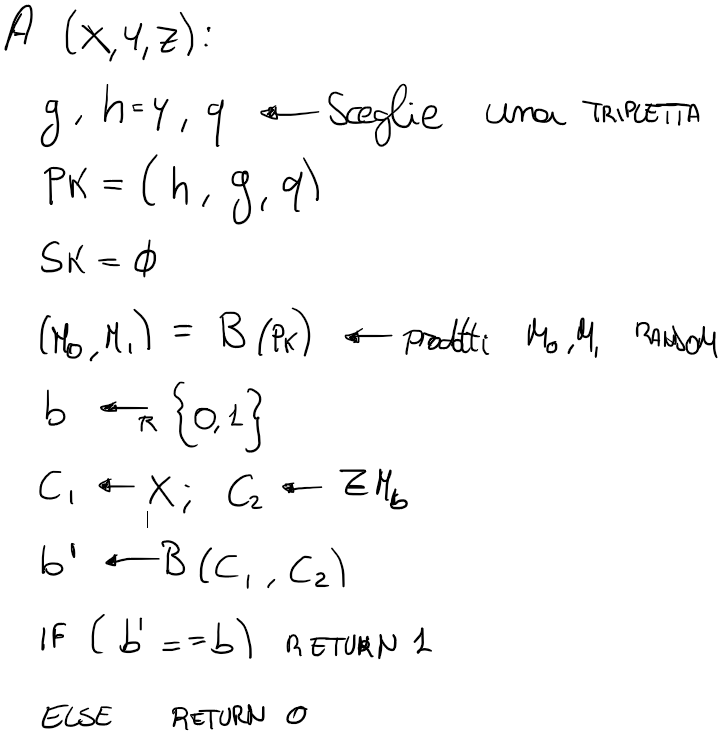
\includegraphics[width=0.4\linewidth]{Images/cifrari_asimmetrici/El_gamal/A_attacco_B.png}
\end{figure}

Cerchiamo di capirlo meglio guardando il vantaggio di A:
\begin{figure}[H]
    \centering
    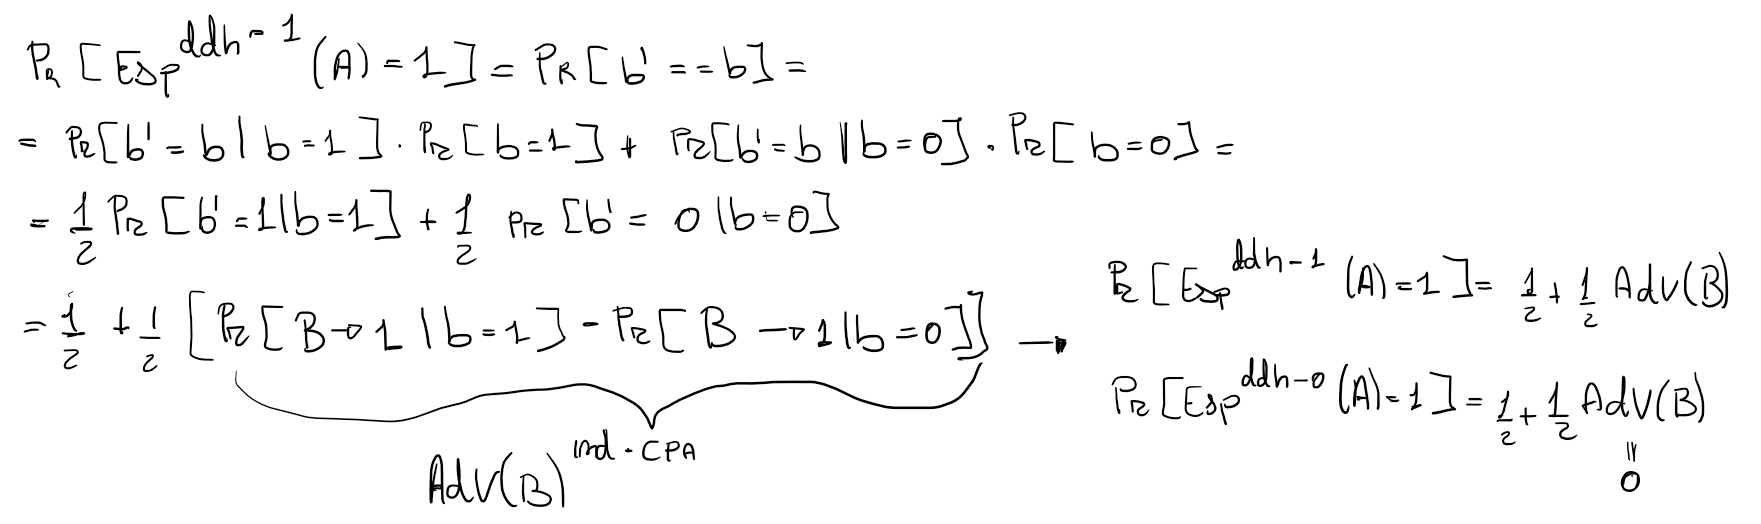
\includegraphics[width=0.9\linewidth]{Images/cifrari_asimmetrici/El_gamal/dim_1.png}
\end{figure}
\begin{figure}[H]
    \centering
    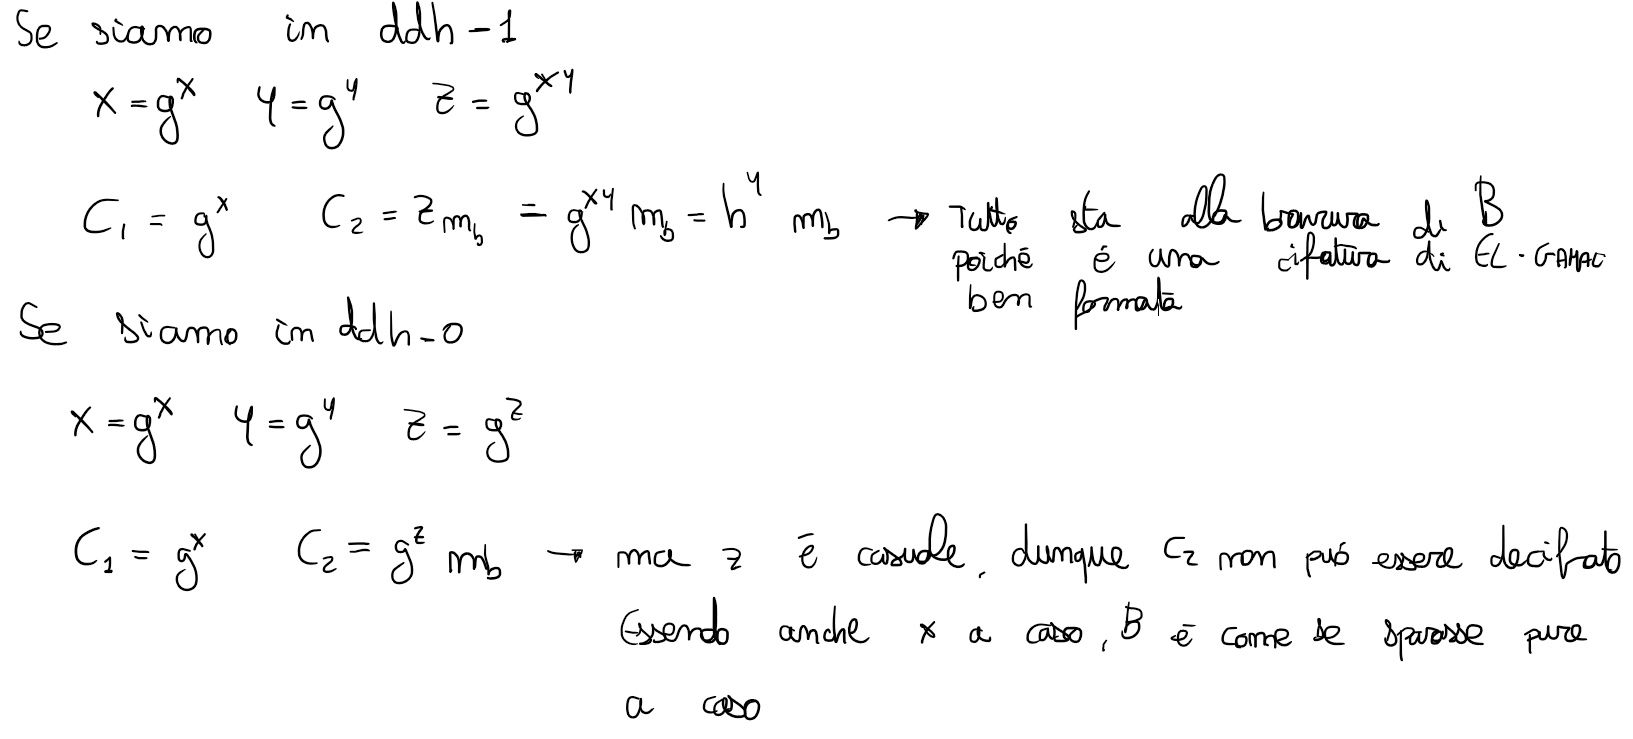
\includegraphics[width=0.9\linewidth]{Images/cifrari_asimmetrici/El_gamal/dim_2.png}
\end{figure}
Per cui, avremo che il vantaggio $Adv(A) = 1/2 Adv(B)$.

Un'altra considerazione da fare è che questo cifrario è \textbf{malleabile}, infatti, possiamo vedere:
\begin{figure}[H]
    \centering
    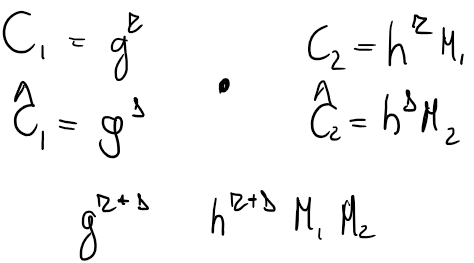
\includegraphics[width=0.3\linewidth]{Images/cifrari_asimmetrici/El_gamal/malleabile.png}
\end{figure}
Tuttavia, possiamo effettuare solo operazioni di moltiplicazione in questo caso. Per rendere possibili le addizioni, abbiamo bisogno di fare alcune modifiche e scendere a compromessi.

\subsection{Lifted El-Gamal}
Sia $B$ piccolo abbastanza da poter effettuare brute-force. Il cifrario Lifted El-Gamal sarà quindi definito così:
\begin{figure}[H]
    \centering
    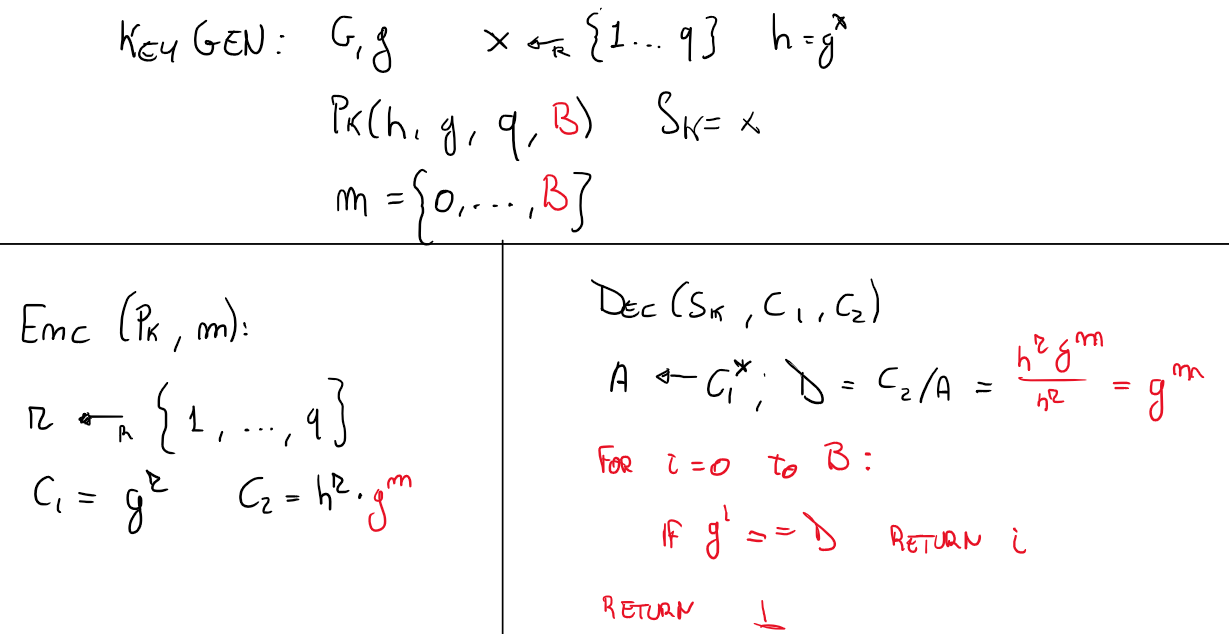
\includegraphics[width=0.7\linewidth]{Images/cifrari_asimmetrici/El_gamal/lifted_elgamal.png}
\end{figure}
Vediamo, infatti:
\begin{figure}[H]
    \centering
    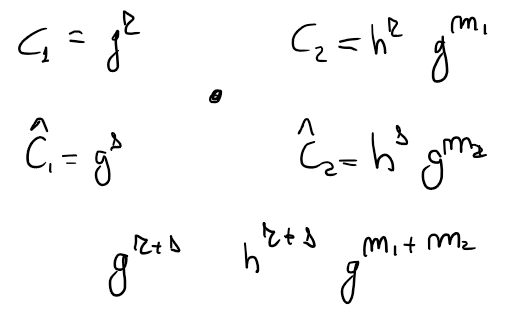
\includegraphics[width=0.3\linewidth]{Images/cifrari_asimmetrici/El_gamal/mall_sum.png}
\end{figure}
\section{Cifrario Pailier}
Passiamo adesso a un cifrario omomorfico che non ha tutte le problematiche che ha Lifted El-Gamal. Questo approccio sarà un ibrido tra una soluzione basata sul logaritmo discreto e una basata sulla fattorizzazione poiché cerca di prendere alcune caratteristiche da ognuno:
\begin{itemize}
    \item \textbf{Logaritmo discreto}: Tramite le soluzioni basate sul logaritmo discreto, riusciamo a ottenere omomorfismo.Tuttavia, non siamo in grado di estrarre $g^{x+y}$. 
    \item \textbf{Fattorizzazione}: Siamo in grado di costruire un sistema trapdoor come RSA. Tuttavia, RSA è moltiplicativo, per cui:
    \[x^e \mod N * y^e \mod N = (xy)^e \mod N\]
\end{itemize}
\subsection{Un po' di Algebra (Ancora...)}
Ricordiamoci che:
\[Z_N* = \{x:0<x<N \cap gcd(x,N)=1\}\]
Dove $N = pq$ con $p,q$ numeri primi. Consideriamo adesso $Z_{N^2}*$ con $N^2 = p^2q^2$. Definiamo adesso x un \textbf{N-Residuo} se $\exists y \rightarrow y^N \mod N^2$ dove y è radice perfetta N-Esima. Supponiamo di prendere l'insieme T sottogruppo di $Z_{N^2}*$. Nello specifico il sottogruppo generato dall'elemento (1+N):
\[T=\{(1+xN)\in Z_{N^2}*: x \in Z_N \}\]
Vediamo che tipo di elementi abbiamo:
\begin{align*}
    & x= 0 \rightarrow 1\\
    & x = N \rightarrow 1+N^2 \mod N^2 = 1
\end{align*}
Andando sul generico, otteniamo:
\begin{align*}
    &(1+xN)^N \mod N^2 = \\
    &= \sum_{i=0}^N \binom{N}{i} (xN)^i \mod N^2 = \\
    &= 1 + \binom{N}{1} xN + \sum_{i=0}^N \binom{N}{i} (xN)^i \mod N^2 = \\
    &= 1+xN^2 + \sum_{i=2}^N \binom{N}{i} (xN)^i = 1 \\
    &\text{Vediamo che $xN^2 = 0$ e $\sum_{i=0}^N \binom{N}{i} (xN)^i = 0$ in quanto tutti multipli di $N^2$ }
\end{align*}
Quindi, possiamo concludere che tutti gli elementi in $T$ sono uguali a 1 in $Z_{N^2}*$. Da qui derivano alcune considerazioni:
\begin{itemize}
    \item Ogni N-residuo ammette N radici N-esime distinte. Cioè se ho $x^N$ questo può derivare da $N$ elementi diversi.
    \item Si consideri l'insieme $T=\{(1+xN)\in Z_{N^2}*: x \in Z_N\}$, ogni elemento in T è tale che $z^N = 1 \mod N^2$.
    \item L'ordine di $Z_{N^2}^{*}$ è $\phi(N^2)$, dunque per ogni x in $Z_{N^2}^{*}$ si ha che $x^{\phi(N^2)}\mod N^2 = 1$.
\end{itemize}
Sappiamo $\phi(N^2)=N\phi(N)$, dunque $x^{\phi(N^2)}=1 \mod N^2$ è equivalente a scrivere $x^{N\phi(N)}=1 \mod N^2$. 
Supponendo di prendere un elemento w che può essere con probabilità $1/2$ un N-Residuo e con probabilità $1/2$ un elemento casuale in $Z_{N^2}^{*}$. Conoscendo la fattorizzazione di N, possiamo capire se questo è un N-residuo seguendo questo algoritmo:
\begin{figure}[H]
    \centering
    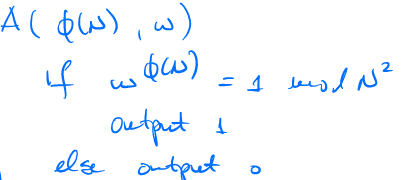
\includegraphics[width=0.5\linewidth]{Images/cifrari_asimmetrici/Pailier/attacco_fattorizzazione.png}
\end{figure} 
Se la fattorizzazione è ignota non esiste nessun algoritmo polinomiale per risolvere questo problema. Possiamo definire il problema della N residuosità decisionale in questo modo:
\begin{figure}[H]
    \centering
    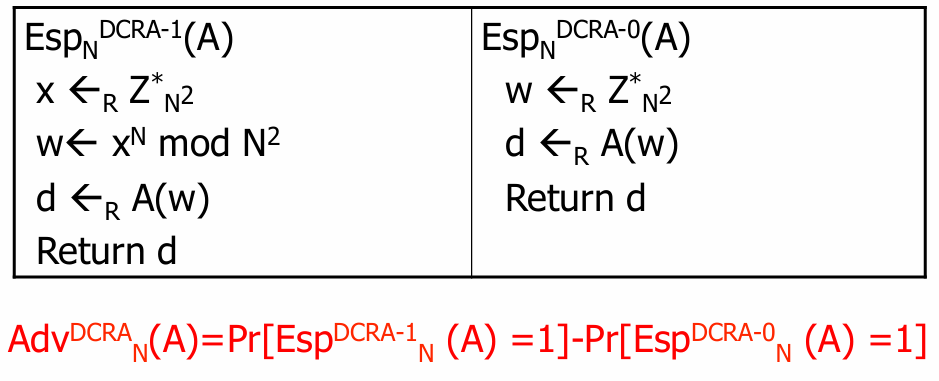
\includegraphics[width=0.7\linewidth]{Images/cifrari_asimmetrici/Pailier/problema_decisionale_N.png}
\end{figure} 
La probabilità che in DCRA-0 si prenda un w che è un elemento residuo è $1/N$, che è praticamente nulla. Si può dimostrare nel seguente modo: l'insieme $Z_{N^2}^{*}$ ha $\phi(N^2) = N \phi(N)$ e la cardinalità degli N-residui è $\phi(N)$. Quindi, casi favorevoli su casi totali arriviamo a $1/N$.\\
Un'ulteriore considerazione è che ogni elemento $w \in Z_{N^2}^{*}$ può essere scritto nella forma $(1+xN)y^N$ con $x \in Z_N$ e $y \in Z_N^{*}$. Sia $Z_{N^2}^{*} \cong Z_N \times Z_N^{*}$ un isomorfismo, fissato $c=(1+N)y^N \mod N^2$, esiste una sola coppia $(x, y)$ che dà quel c.
\subsection{Algoritmo di Cifratura}
Innanzitutto definiamo l'algoritmo di generazione della chiave. Questo è molto simile a RSA, generiamo $p,q$ primi a caso e calcoliamo $N=pq$.Scegliamo come chiave pubblica $N$ e come chiave privata la coppia $(p,q)$, cioè la fattorizzazione di N. Lo spazio dei messaggi è $Z_N$ e lo spazio dei crittotesti è $Z_{N^2}^{*}$.

L'algoritmo di cifratura è, invece, il seguente:
\begin{figure}[H]
    \centering
    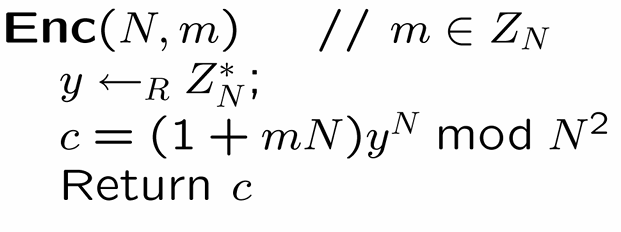
\includegraphics[width=0.4\linewidth]{Images/cifrari_asimmetrici/Pailier/encryption.png}
\end{figure} 
Più complicata è la decifratura dei messaggi. Cerchiamo di dividere la cosa in più passi:
\begin{enumerate}
    \item Calcoliamo:
        \begin{align*}
            c^{\phi(N)}=\\
            & = ((1+mN)y^N)^{\phi(N)} \mod N^2 =\\
            & = (1+mN)^{\phi(N)}y^{N\phi(N)} \mod N^2 =\\
            & = (1+mN)^{\phi(N)}
        \end{align*}
    In questo modo, togliendo y, abbiamo tolto la randomness.
    \item Ogni elemento $(1+xN)$ ha ordine N in $Z_{N^2}^{*}$. Dunque, poiché $gcd(N, \phi(N))=1$, esiste $d$ tale che $d\phi(N)=1 \mod N$.
    \[C = (c^{\phi(N)})^d = (1+mN)^{\phi(N)d}\mod N^2 = (1+mN)\mod N^2 \]
    Il fatto che $d\phi(N)=1 \mod N$, vuol dire che $d\phi(N)=1+kN$. Posso scomporre $(1+mN)^{1+kN}=(1+mN)*((1+mN)^N)^k = (1+mN)$.
    \item Infine, possiamo calcolare m da c nel seguente modo:
    \[m=\frac{C-1}{N}\] 
\end{enumerate}

Vediamo come questo cifrario è malleabile e come si possa fare la somma: 
\begin{figure}[H]
    \centering
    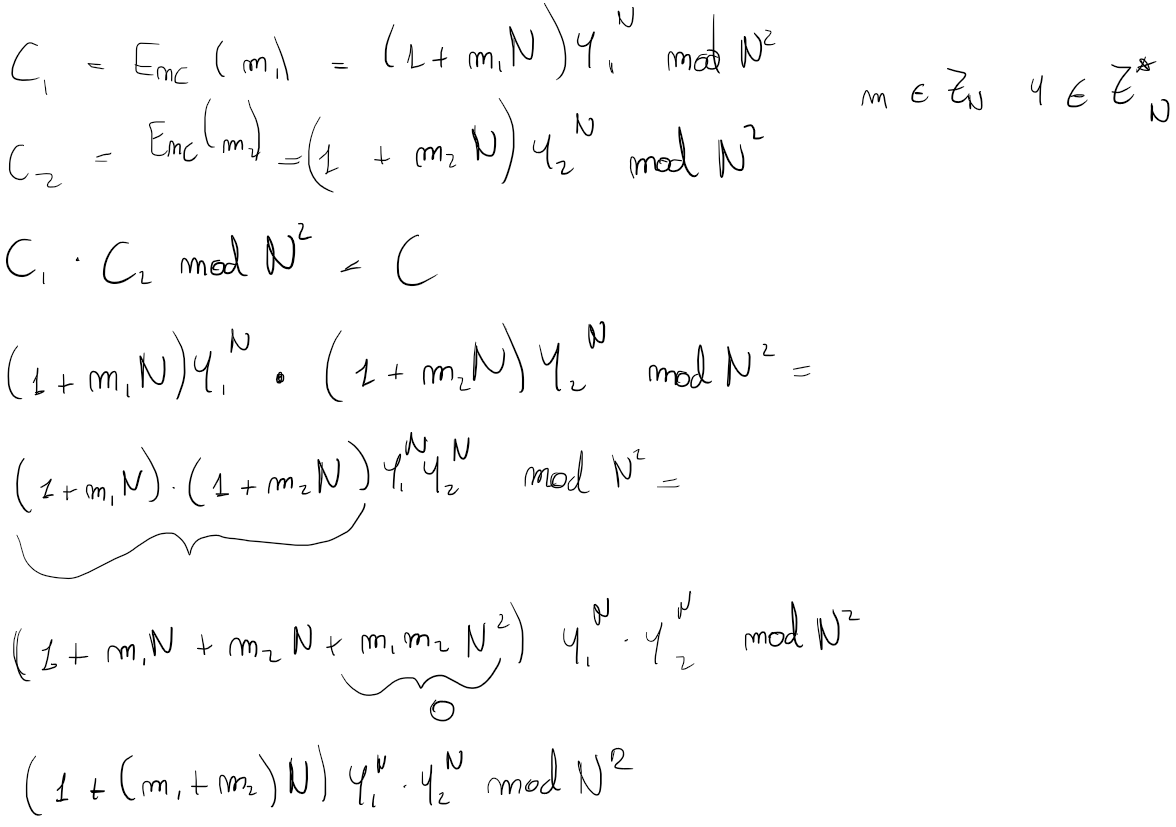
\includegraphics[width=1\linewidth]{Images/cifrari_asimmetrici/Pailier/mall_1.png}
\end{figure} 
Notiamo come la prima parte abbia effettivamente la somma:
\begin{figure}[H]
    \centering
    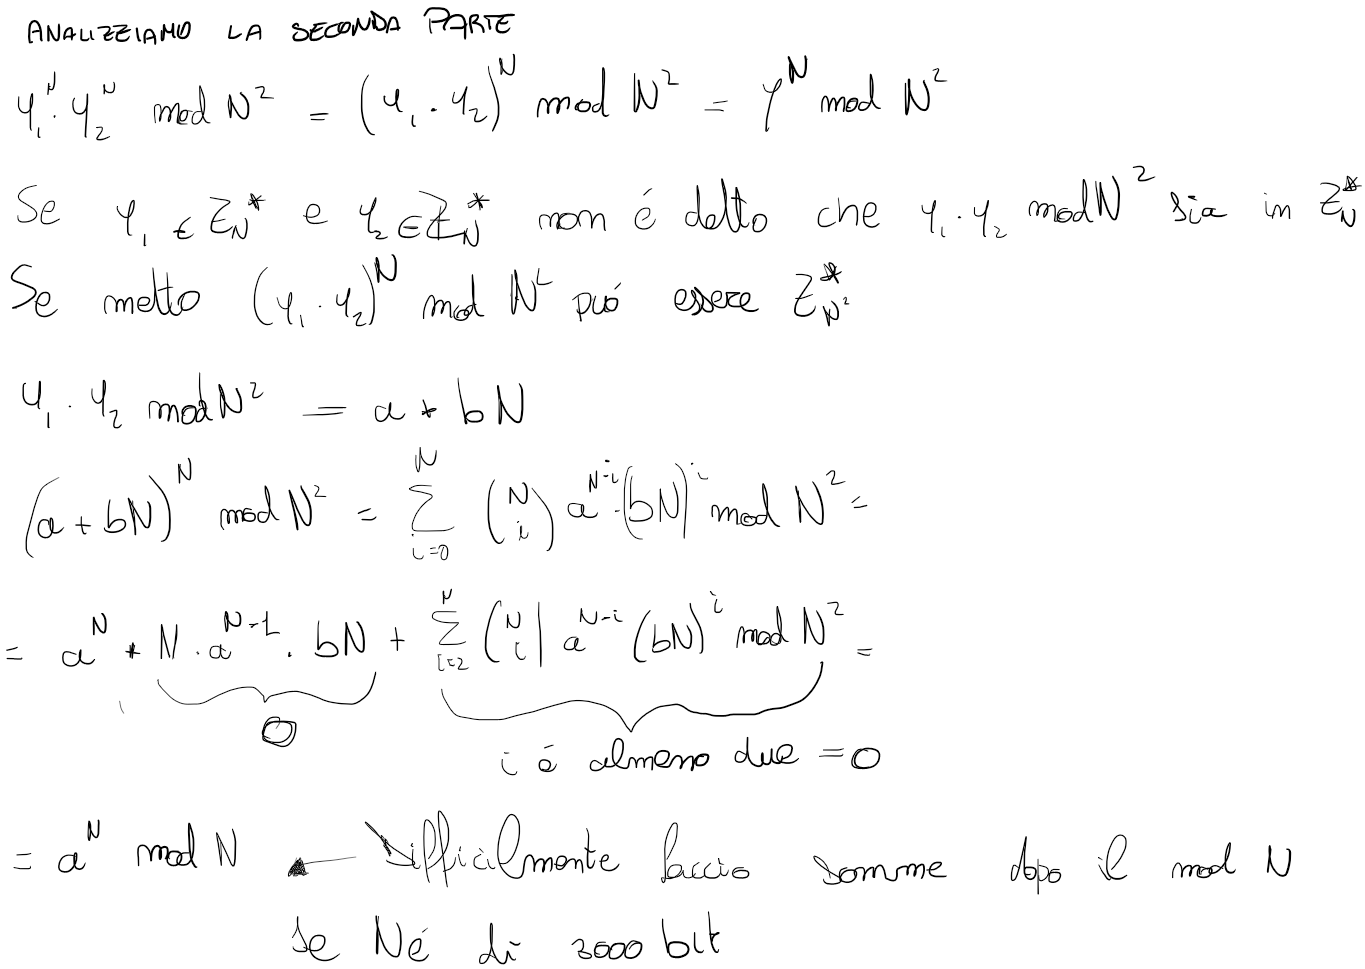
\includegraphics[width=1\linewidth]{Images/cifrari_asimmetrici/Pailier/mall_2.png}
\end{figure} 
Adesso che siamo riusciti a fare la somma, vediamo come fare la moltiplicazione per una costante:
\begin{figure}[H]
    \centering
    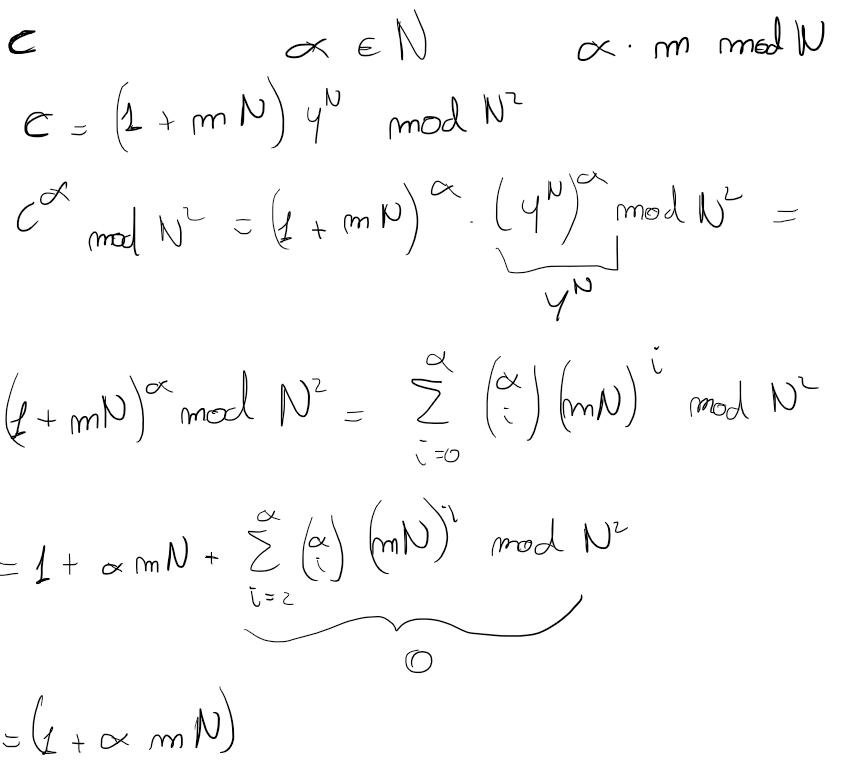
\includegraphics[width=0.6\linewidth]{Images/cifrari_asimmetrici/Pailier/mall_3.png}
\end{figure} 

\subsection{Elezione Multi-Candidato}
Supponiamo di avere quattro candidati in un sistema di elezione che chiameremo $C_1,\dots, C_4$ e vogliamo che vi sia segretezza nel voto ma che sommando tutti i voti ci venga fornito il risultato delle elezioni. Sappiamo che lo spazio dei messaggi è $Z_N$ con $N=pq$, immaginando che $N=2000$, possiamo creare un array di questo tipo:
\begin{figure}[H]
    \centering
    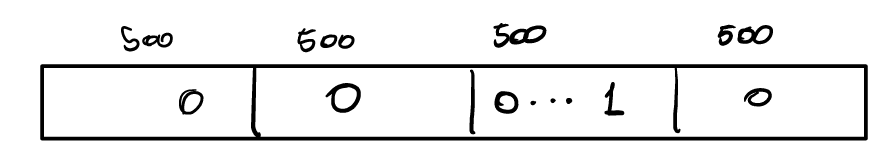
\includegraphics[width=0.5\linewidth]{Images/cifrari_asimmetrici/elezione_multi-candidato.png}
\end{figure} 
In questo modo, dividiamo l'array in quattro sezioni e ogni voto si va' a sommare in quella specifica sezione. Questo sistema, così come proposto, non è funzionante poiché presuppone che tutti gli elettori siano onesti. Tuttavia, vi sono dei modi per far sì che questo sistema funzioni.

\section{Cifrari RSA-OAEP}
Fino a ora abbiamo presentato tutti cifrari sicuri contro avversari CPA ma che crolla in contesti CCA. Passiamo adesso a un cifrario sicuro contro attacchi CCA noto come \textbf{RSA-OAEP} che è l'attuale standard di sicurezza anche se, in questi ultimissimi anni, si sta passando ai cifrari post-quantum.
Questo cifrario è sicuro se considerato nel contesto \textbf{Random Oracle Model} in cui abbiamo la necessità di un oracolo di Hash che preso in input $x$ ritorna il suo hash in maniera tale che sia del tutto casuale. La nostra ipotesi è che se sostituiamo a questo oracolo una vera funzione Hash, il cifrario rimanga sicuro. Questa ipotesi è, però, falsa; tuttavia, tutti i controesempi trovati sono molto artificiali e del tutto impraticabili. 
La difficoltà nel costruire cifrari sicuri contro attacchi a crittotesto scelto è dovuta principalmente a due cause:
\begin{enumerate}
    \item Il simulatore deve essere in grado di decifrare senza risolvere il problema computazionale alla base della sicurezza del sistema.
    \item Dobbiamo impedire all'attaccante di creare crittotesti utili a partire da quello sul quale lo sfidiamo.
\end{enumerate}
Prima di iniziare con il cifrario vero e proprio, diamo alcune definizioni:
\begin{itemize}
    \item k è la "taglia" del modulo RSA in uso.
    \item $k_0,k_1$ sono dei parametri tali che $k_0+k_1<k$.
    \item Lo spazio dei messaggi è composto da tutte le stringhe di lunghezza $n$ dove $n=k-k_0-k_1$.
    \item Siano 
    \begin{itemize}
        \item $G:\{0,1\}^{k_0}\rightarrow \{0,1\}^{n+k_1}$
        \item $H:\{0,1\}^{n+k_1} \rightarrow \{0,1\}^{k_0}$
    \end{itemize}
    Due random oracle.
\end{itemize}
Cominciamo a vedere gli algoritmi di generazione della chiave, di cifratura e decifratura. L'algoritmo di generazione della chiave è, banalmente, lo stesso algoritmo utilizzato per RSA.  

Per quanto riguarda l'algoritmo di cifratura, avremo invece:
\begin{figure}[H]
    \centering
    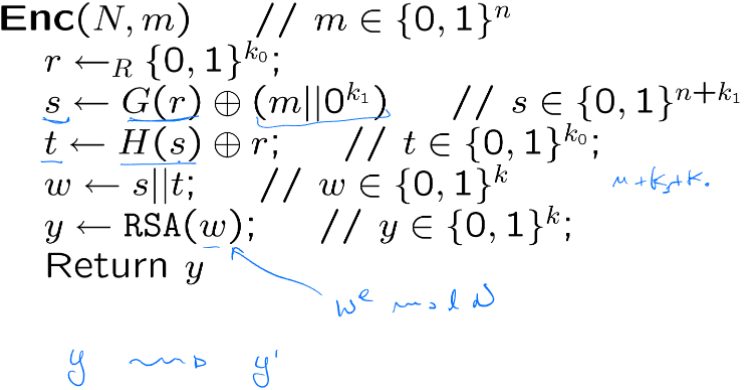
\includegraphics[width=0.7\linewidth]{Images/cifrari_asimmetrici/RSA-OAEP/encrypt.png}
\end{figure} 
Il costo di questa operazione è molto basso, praticamente la cosa più costosa è l'elevazione causata dall'utilizzo di RSA. Il vero problema è che in termini di banda, non possiamo fare molto di meglio poiché, supponendo di voler mandare solo 256 bit, ne manderemo 3000. Tuttavia diciamo che ci accontentiamo poiché, come già detto precedentemente, quello che facciamo è utilizzare la crittografia asimmetrica solo per scambiare una chiave simmetrica. Dunque, una volta scambiata la chiave simmetrica, la cifratura asimmetrica non viene più utilizzata. 

Infine, per quanto riguarda l'algoritmo di decifratura abbiamo:
\begin{figure}[H]
    \centering
    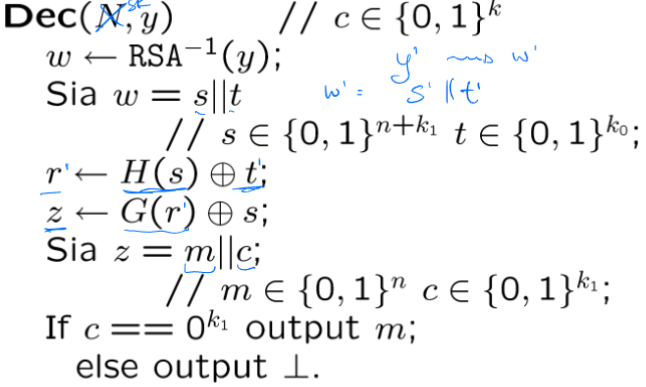
\includegraphics[width=0.7\linewidth]{Images/cifrari_asimmetrici/RSA-OAEP/decrypt.png}
\end{figure} 
Come possiamo notare, riusciamo effettivamente a decifrare il messaggio e il padding precedentemente effettuato. Proprio su quest'ultimo viene effettuato un ulteriore controllo, poiché con una probabilità molto alta, se viene effettuata una modifica al crittotesto, questo andrà a modificare anche quella stringa di zeri trasformandone almeno uno.

Una volta visto che questo sistema è sicuro (non lo dimostriamo poiché troppo complicato), non ci rimane altro che gestire correttamente il sistema delle chiavi pubbliche. Tendenzialmente, viene adottato il sistema \textbf{Public Key Infrastructure}, una struttura di chiavi che certificano che una data chiave pubblica appartiene a una specifica persona/identità. Questa struttura è parecchio complessa e si arriva ricorsivamente a dover verificare l'autenticità dell'autenticità ecc. fino ad arrivare alla così dette \textbf{root key} che sarebbe una chiave auto certificata. Per ottenere la certificazione è necessaria una procedura burocratica atta a questo scopo.

\section{Identity Based Encryption}
Per ovviare al problema della certificazione della chiave, quello che vorremmo fare è sfruttare procedure burocratiche già esistenti per ottenere una chiave pubblica. Ad esempio, ipotizziamo che la procedura d'iscrizione all'università rilasci una mail universitaria e supponiamo di voler utilizzare quest'ultima come chiave pubblica. Questo sistema viene definito \textbf{Cifratura basata sull'identità}. Rendiamoci conto dei vantaggi che questo sistema può offrire:
\begin{itemize}
    \item La mail è facilmente riconoscibile, non c'è il rischio di confondere una "chiave" da un'altra.
    \item Posso creare delle chiavi pubbliche a "scadenza" ad esempio generando una mail seguita dall'anno di validità.
    \item Posso inviare messaggi senza che il destinatario abbia già generato la sua chiave.
\end{itemize}

Tuttavia, rimane il problema della generazione della chiave privata. Per fare ciò, abbiamo bisogno di un \textbf{segreto master} da cui poter generare le chiavi private a partire dalle chiavi pubbliche. In questo modo, riusciremo a risolvere anche il problema di \textbf{key escrow}, cioè il fatto che, in certi casi particolari (come ad esempio i casi di procedura penale), voglio far sì che un ente terzo possa rompere la cifratura. Questo viene risolto poiché basterebbe che l'ente di generazione generi nuovamente la chiave privata dell'utente e la dia alla corte penale. Rimane però il fatto che, dando questa possibilità, non è detto che non ne venga abusato. Inoltre, possiamo immaginare quanto possa essere dannoso uno scenario in cui venga compromessa la chiave master.
\subsection{Schema Boneh-Franklin}
Questo sistema di cifratura sfrutta mappe \textbf{bilineari} tra due gruppi $G_1, G_2$ in cui il problema Diffie-Hellman è intrattabile. Avremo, quindi, un \textbf{Trusted-Third-Party} che genera le chiavi private degli utenti. Vediamo i requisiti di sicurezza che vogliamo ottenere oltre quelli classici:
\begin{enumerate}
    \item Vogliamo far sì che se non si conosce la master key, non si possa generare la chiave privata.
    \item Vogliamo far sì che due utenti o più collusi non possano generare un'altra chiave che non gli appartiene.
\end{enumerate}
Vediamo quindi la definizione \textbf{ind-id-cpa}:
\begin{figure}[H]
    \centering
    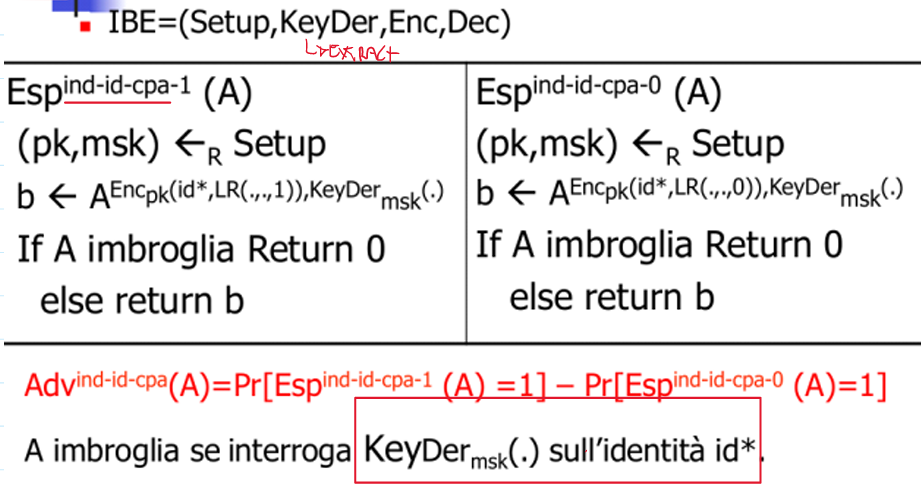
\includegraphics[width=0.7\linewidth]{Images/cifrari_asimmetrici/Boneh-Franklin/ind_id_cpa.png}
\end{figure} 
In cui A può accedere a un oracolo di estrazione che prende in input un id e ne restituisce la chiave privata e a un oracolo di cifratura che prende una stringa e la cifra con l'id su cui A vuole essere sfidato.

Siano $G_1,G_2,G_t$ dei gruppi con le seguenti proprietà:
\begin{enumerate}
    \item $G_1,G_2$ sono gruppi di ordine q primo e $G_1$ è generato da $P$ e $G_2$ da $P'$.
    \item Esiste un isomorfismo $\rho:G_2 \rightarrow G_1, \rho(P') = P$
    \item Esiste una mappa bilineare $e:G_1 \times G_2 \rightarrow G_T$
\end{enumerate}
Una mappa si dice \textbf{Bilineare} se $\forall U \in G_1, V \in G_2, (a,b) \in Z: e(U^a, V^b) = e(U,V)^{ab}$. La mappa non deve nemmeno essere \textbf{degenere}, cioè non deve succedere che $e(P,P')=1_{G_T}$. Un esempio di mappa bilineare è il prodotto scalare.

Ma vediamo adesso il cifrario in sé per sé. Questo si compone di quattro algoritmi: \textbf{Setup, Key Extraction, Encryption e Decryption}. Vediamoli uno a uno:
\begin{itemize}
    \item \textbf{Setup}: Questo sceglie il master secret key uniformemente a caso in $[1,\dots,q]$. La chiave pubblica sarà $Pk = (P')^{msk}$.
    \item \textbf{KeyExtraction}: la chiave segreta dell'utente id sarà $P_{id} = H_1 (id)$ e poi $usk = P_{id}^{msk}$. Con $H_1$ che manda stringhe di bit di lunghezza arbitraria in $G_1$. 
    \item \textbf{Cifratura}: L'algoritmo funziona nel seguente modo:
        \begin{figure}[H]
            \centering
            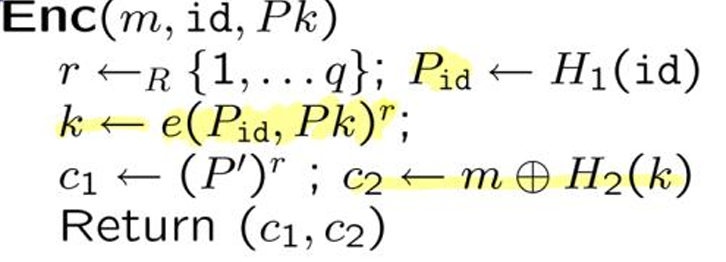
\includegraphics[width=0.5\linewidth]{Images/cifrari_asimmetrici/Boneh-Franklin/enc.png}
        \end{figure} 
    Con $H_2$ che manda $G_T$ in stringhe di bit di lunghezza arbitraria.
    \item \textbf{Decifratura}: infine, vediamo l'algoritmo di decifratura:
        \begin{figure}[H]
            \centering
            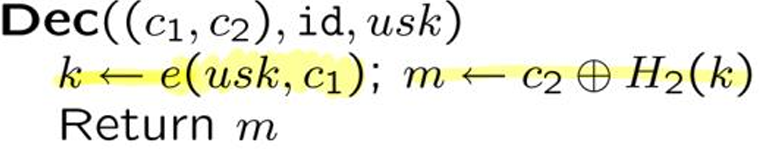
\includegraphics[width=0.5\linewidth]{Images/cifrari_asimmetrici/Boneh-Franklin/dec.png}
        \end{figure} 
\end{itemize}
Possiamo dimostrare la correttezza di questo algoritmo:
\begin{figure}[H]
    \centering
    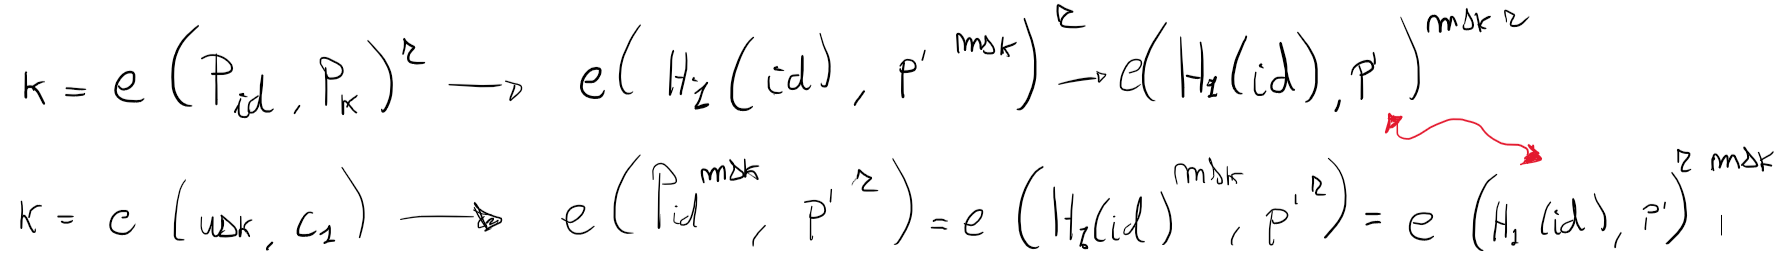
\includegraphics[width=0.7\linewidth]{Images/cifrari_asimmetrici/Boneh-Franklin/correttezza.png}
\end{figure} 
Per quanto riguarda, invece, la dimostrazione di sicurezza di questo cifrario, utilizziamo il \textbf{problema DDH bilineare}, per cui:
\begin{figure}[H]
    \centering
    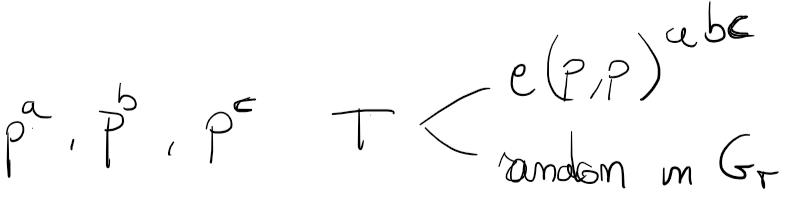
\includegraphics[width=0.5\linewidth]{Images/cifrari_asimmetrici/Boneh-Franklin/sicurezza.png}
\end{figure} 
Dove l'obiettivo è quello di capire se T è $e(P,P)^{abc}$ o un elemento a caso in $G_T$. Si può dimostrare che il problema BDH può essere risolto se viene risolto il problema CDH.\footnote{Computational Diffie-Hellman}
\begin{figure}[H]
    \centering
    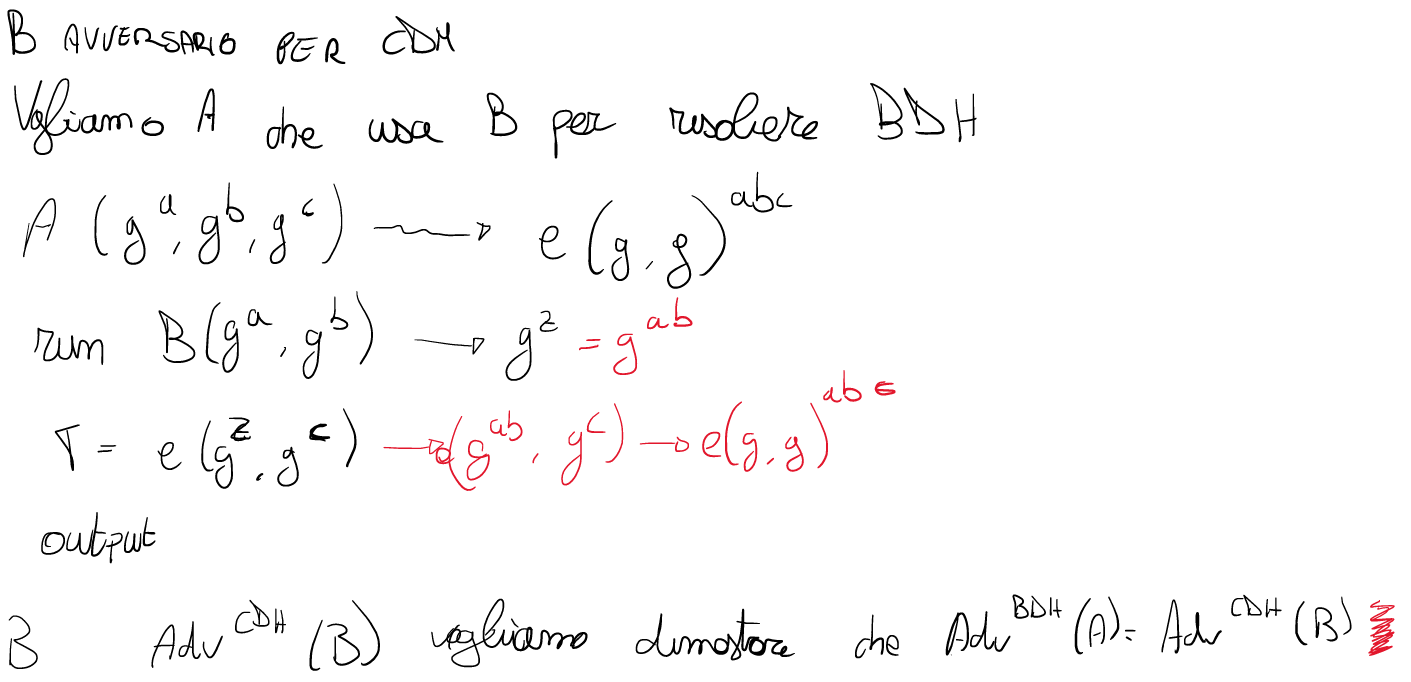
\includegraphics[width=0.8\linewidth]{Images/cifrari_asimmetrici/Boneh-Franklin/bdh_cdh.png}
\end{figure} 


